\newcommand{\titreA}{Solution efficiente pour la s\'{e}curisation des r\'{e}seaux d'entreprise}
\newcommand{\titreB}{Rapport de projet industriel}
\documentclass[12pt]{article}
\usepackage[utf8]{inputenc}
\usepackage[francais]{babel}
\usepackage[T1]{fontenc}
\usepackage{lmodern, marvosym, geometry, graphicx, multicol, lastpage, tikz, listings}
\usepackage[hyperindex=true, colorlinks=true, breaklinks=true, linkcolor=blue]{hyperref}
\usepackage{fancyhdr, verbatim, alltt, pdfpages}

\geometry{hmargin=1.5cm, vmargin=2cm}
\addtolength{\parskip}{10pt}
\pagestyle{fancy}

\definecolor{lightgray}{gray}{0.9}
\definecolor{darkgray}{gray}{0.4}
\newcommand{\hlc}[1]{\color{purple}{\textbf{#1}}}
\lstset{language=,
    basicstyle=\sffamily\footnotesize,
    xleftmargin=20pt,
    xrightmargin=20pt,
    numbers=left,
    stepnumber=1, % le pas des numeros de ligne
    numbersep=10pt,
    breaklines=true,
    tabsize=4,
    %frame=single,
    showspaces=false,
    showstringspaces=false
    inputencoding=utf8, %put1 d'utf8 dans listing
    extendedchars=true, %put1 d'utf8 dans listing
    literate={à}{{\`a}}1 {é}{{\'e}}1 {è}{{\`e}}1 {ê}{{\^e}}1 {â}{{\^a}}1 {î}{{\^i}}1 {ê}{{\^e}}1 {É}{{\'E}}1 {À}{{\`A}}1 {«}{{\og}}1 {»}{{\fg{}}}1 {ô}{{\^o}}1 {ù}{{\`u}}1 {û}{{\^u}}1 {ç}{{\c{c}}}1 {Ç}{{\c{C}}}1 {--}{{-\,-}}1 {-}{{-}}1 {*}{{*}}1 {Switch(config)\#}{{\textbf{Switch(config)\# }}}1 {Switch(config-if)\#}{{\textbf{Switch(config-if)\# }}}1 {Switch(config-line)\#}{{\textbf{Switch(config-line)\# }}}1 {Switch>}{{\textbf{Switch> }}}1 {Switch\#}{{\textbf{Switch\# }}}1, %put1 d'utf8 dans listing
    columns=fullflexible, % suppression des espaces autour des deux-points
    escapechar=§, % permet d'insérer du §code latex§
    backgroundcolor=\color{lightgray},
    alsoletter={.,1,2,3,4,5,6,7,8,9,0},
    keywords={path_to_certs, user_login, user_password, nom_entreprise, pass_radius_sql, utilisateur1, pass_utilisateur1, secret_radius, 192.168.1.2, 192.168.1.10, 255.255.255.0, fastethernet0/1, vlan_id, pass_enable, pass_enable_secours, utilisateur_secours, pass_utilisateur_secours, pass_root_sql, snack, 192.168.0.254, commutateur1, client1, Nancy, BHConsulting, France, FR, nom_serveur_radius, dossier_certs, dossier_certs_utilisateur, eth0 },
    keywordstyle=\hlc,
    morecomment=[l]{\#}, % commentaires shell en ligne
    commentstyle=\itshape\color{darkgray},
}

\renewcommand{\headrulewidth}{1pt}
\lhead{\textbf{\titreA{} (\titreB)}}
\rhead{\emph{BOUGET / GUÉPIN / PINHÈDE / VAUBOURG}}
\lfoot{TELECOM Nancy - PI}
\cfoot{\thepage{} / \pageref{LastPage}}
\rfoot{2012-2013}

\begin{document}
\thispagestyle{empty}

\begin{multicols}{2}
{\large
	\begin{flushleft}
		\noindent{}\textbf{Nicolas BOUGET}\\
		\Letter~nicolas.bouget@esial.net\\
		3A TRS1\\~

		\noindent{}\textbf{Julien GUÉPIN}\\
		\Letter~julien.guepin@esial.net\\
		3A IL\\
	\end{flushleft}

	\begin{flushright}
		\noindent{}\textbf{Marc PINHÈDE}\\
		\Letter~marc.pinhede@esial.net\\
		3A LE\\~

		\noindent{}\textbf{Julien VAUBOURG}\\
		\Letter~julien@vaubourg.com\\
		3A TRS2\\
	\end{flushright}
}
\end{multicols}

\vspace{0.5cm}

\begin{center}
	{\Huge\textbf{\titreA}}

	\vspace{1cm}

	{\huge\emph{\titreB}}

	\vspace{1cm}

	\begin{flushleft}
		{\large
		\hspace{3.2cm}
		\textbf{Société~:} B.H. Consulting\\
		\hspace{3.2cm}
		\textbf{Intervenant industriel~:} Guillaume ROCHE\\
		\hspace{3.2cm}
		\textbf{Intervenant universitaire~:} Jean-François SCHEID
		}
	\end{flushleft}

	\vspace{1cm}
	{\large Le \today}

	\vspace{1.5cm}

	
\includegraphics[width=140pt]{img/BHConsulting.jpg}

	\vspace{1.5cm}

	
\includegraphics[width=190pt]{img/ul.png}
	\hspace{3.5cm}
	
\includegraphics[width=140pt]{img/telecom-nancy.jpg}
\end{center}
\newpage

\thispagestyle{empty}
\tableofcontents
\newpage



\listoffigures
\newpage

\section{Introduction}
\subsection{Préambule}

Le travail décrit dans ce document est réalisé dans le cadre des projets industriels de la dernière année de la formation ingénieure de l'école TELECOM Nancy. Ce module s'effectue sur une durée de six mois, en partenariat avec l'entreprise B.H. Consulting. Jean-François SCHEID, maître de conférences et enseignant à l'école, a accepté d'encadrer le projet en tant qu'intervenant universitaire.

L'entreprise rémunère l'école pour le travail effectué en deux paiements, dont le second dépend de sa satisfaction à la vue du travail effectué. L'équipe du projet est constituée de quatre étudiants, qui s'engagent à travailler 1000 heures, soit 250 heures par personne.

Un rapport et une soutenance sont présentés à mi-parcours du projet, pour un rendu final en fin d'année scolaire.

\subsection{TELECOM Nancy}

TELECOM Nancy, école associée de l'Institut Mines-Télécom, est une école d'ingénieurs publique de l'Université de Lorraine. Il s'agit d'une école généraliste en informatique, sciences et technologies du numérique, habilitée par la Commission des Titres d'Ingénieurs (CTI). Elle fait partie du Concours TELECOM INT, et a changé de nom au début de l'année 2012, se faisant connaître jusqu'alors sous le nom de ESIAL.

En plus d'un tronc commun, elle dispose de quatre spécialisations différentes, qui vise quatre domaines distincts~:

\begin{description}
\item[Ingénierie du Logiciel~:] Développement d'applications sûres et robustes, avec un attachement particulier pour le domaine du web.
\item[Logiciels Embarqués~:] Étude des systèmes embarqués et programmation efficace dans des environnements restreints.
\item[Systèmes d'Information d'Entreprise~:] Étude des systèmes d'information et des bases de données.
\item[Télécommunications, Réseaux et Services~:] Étude du fonctionnement et de la gestion des réseaux informatiques.
\end{description}

\subsection{B.H. Consulting}

Initialement crée par Bertrand PÉTAT (gérant actuel) en 2000 dans la région luxembourgeoise, B.H. Consulting s'est importée en France dès 2001. Située à Nancy, l'entreprise est restée en contact avec beaucoup de clients luxembourgeois et continue donc d'assurer ses prestations au Luxembourg, comme en France.

Elle comprend quatre employés et un gérant~:

\begin{itemize}
\item Bertrand PÉTAT (gérant)
\item Christine MARCILLAT (secrétaire de direction)
\item Guillaume ROCHE (ingénieur réseau)
\item Jérémy KRAEMER (ingénieur réseau)
\item Simon KOSMERL (ingénieur réseau)
\end{itemize}

L'organigramme est disponible en figure~\ref{organigramme} page~\pageref{organigramme}.

\begin{figure}[!h]
	\begin{center}
		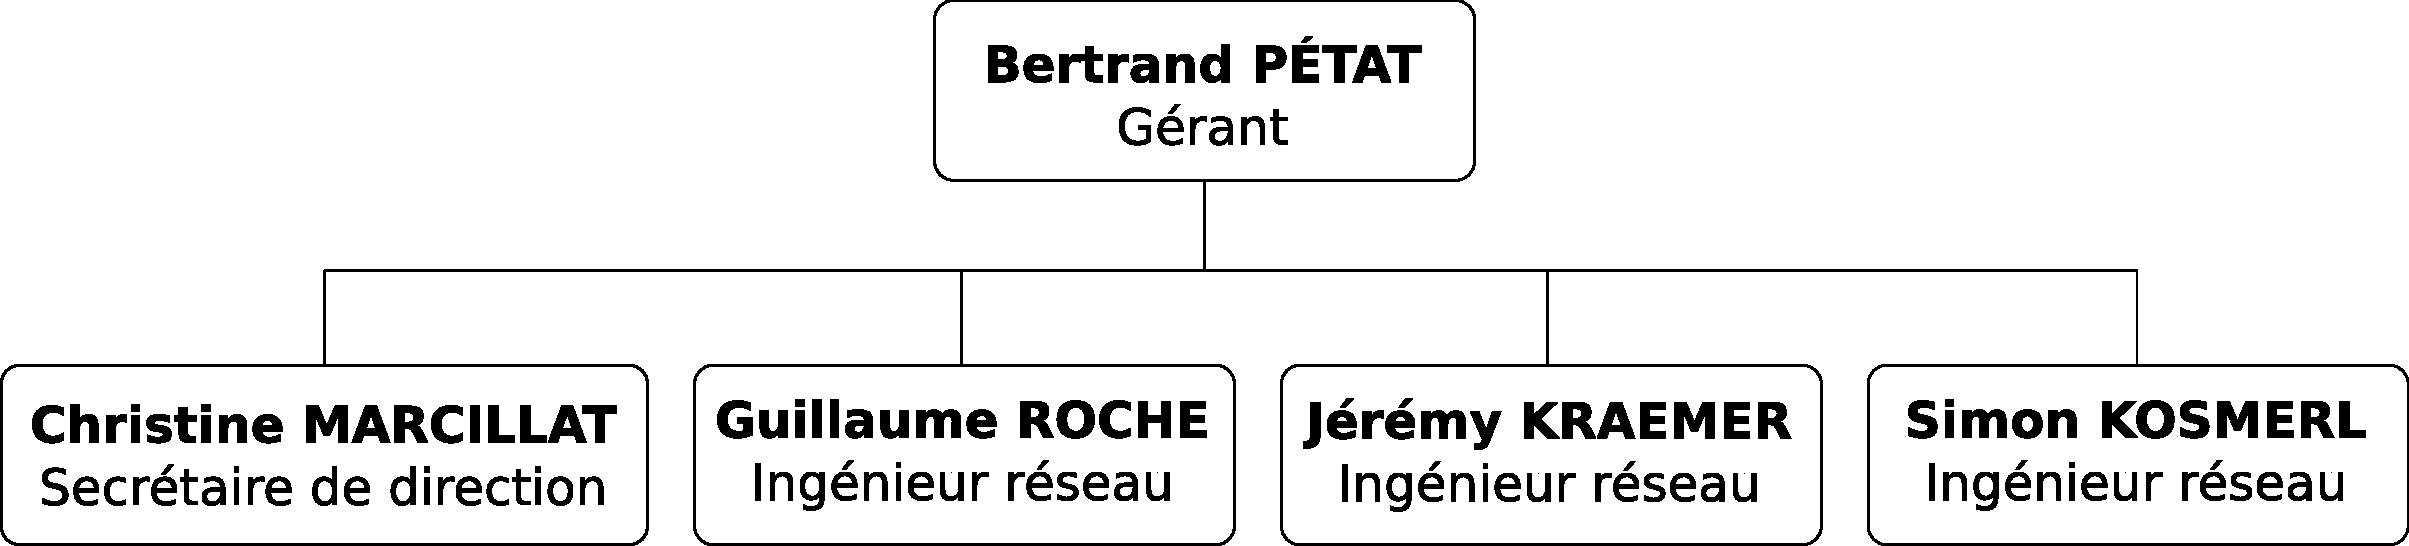
\includegraphics[width=\textwidth]{img/organigramme.pdf}
	\end{center}
	\caption{Organigramme de B.H. Consulting}
	\label{organigramme}
\end{figure}

B.H. Consulting est spécialisée dans les services d'intégration réseau pour les entreprises. Aux côtés de partenaires comme Cisco (équipements réseaux) et Astaro (sécurité), elle conseille et assure l'élaboration d'architectures réseau dans les domaines de l'informatique, de la téléphonie et de la vidéosurveillance. Elle propose des prestations pour des réseaux locaux \og~sur mesure\fg{} selon les attentes du client (adresses IP, sécurité, fiabilité, qualité de service, évolutivité, etc.).

L’entreprise offre un service global qui va de l’étude de cas jusqu’à la mise en oeuvre du réseau et sa maintenance.

Elle propose les prestations suivantes~:

\begin{description}
\item[Proposition de solution~:] Tests et validation des configurations au préalable sur maquette, exposition du choix à l’utilisateur final et décision d’un plan de migration d’architecture.
\item[Mise en oeuvre~:] Configuration, installation et câblage avec le minimum de gêne et de temps d’interruption pour l’activité de l’entreprise.
\item[Analyse fonctionnelle~:] Étude des besoins et des fonctions souhaitées par l’utilisateur compte tenu de son activité, détermination des solutions possibles.
\item[Audit visuel du réseau existant~:] Inventaire informatique, mise en évidence des défauts de câblages, des failles de sécurité ou de fiabilité, des problèmes techniques (alimentation électrique, ventilation), etc.
\item[Maintenance~:] Résolution des différents problèmes rencontrés par l’utilisateur au cours de l’exploitation.
\end{description}

\section{Projet}
\subsection{Contexte}

La sensibilisation croissante aux notions de sécurisation des réseaux des entreprises a conduit B.H. Consulting à devoir répondre à de nouveaux types d'exigences.

Les réseaux d'une entreprise sont en effet devenus un point critique de toutes les nouvelles sociétés, qui sont régulièrement amenées à perdre des heures considérables de travail dès lors que ceux-ci ne sont plus accessibles. Au-delà de l'aspect fonctionnel, les réseaux sont des accès particulièrement critiques pour les serveurs les plus sensibles des administrations, qui stockent les informations les plus confidentielles d'une entreprise.

Qu'ils soient filaires ou non, ces réseaux sont accessibles dès lors qu'on est dans les locaux des entreprises~: prises murales, émissions wifi, etc. N'importe quel individu ayant alors la possibilité de se relier physiquement aux réseaux, il faut mettre en place un mécanisme de contrôle logique pour restreindre ses accès. Pour autant, ce mécanisme ne doit pas être lourd à administrer, ce qui impliquerait rapidement un laxisme et une confusion dans les règles établies. Définir strictement les autorisations en fonction des points d'accès physiques, pour ensuite établir une carte des autorisations de l'ensemble des bâtiments n'est pas non plus la bonne solution, puisqu'il sera difficile de garantir les contrôles d'accès à ces prises. L'utilisation du réseau dépendra également de l'emplacement géographique de l'utilisateur, à l'encontre de toute logique vis-à-vis de la tendance actuelle au nomadisme constaté dans les entreprises.

Pour répondre à toutes ces exigences, critiques pour une entreprise qui souhaite garantir l'intégrité de son réseau et la confidentialité de ses données (tout en sauvegardant la liberté de mouvement de ses employés), B.H. Consulting est régulièrement contraint d'exploiter les nouvelles technologies les plus adéquates. De nouveaux outils d'administration doivent donc être régulièrement développés pour pouvoir être proposés à ses clients.

Au delà du déploiement des politiques de sécurisation, B.H. Consulting souhaite offrir une souplesse d'administration exemplaire de son système, en permettant aussi bien à ses clients que ses propres employés de modifier aisément les permissions des réseaux. Aucune des solutions d'interface existantes ne semble répondre à ce besoin actuellement. En plus d'une interface accessible, ergonomique et complète, B.H Consulting souhaiterait proposer des fonctionnalités poussées comme la gestion d'un historique, des équipements actifs ou encore une console virtuelle.

Les objectifs de ce projet industriel émanent directement des besoins des clients, auxquels B.H. Consulting doit faire face.

\subsection{Objectifs}

Plusieurs objectifs peuvent être déduits du contexte.

La première étape majeure du projet sera donc~:

\begin{enumerate}
\item Déterminer la technologie qui permettra de définir des accès aux réseaux de façon dynamique, souple et sécurisée.
\item Former l'équipe du projet industriel sur cette technologie, à l'aide de documentations et d'expérimentations concrètes sur les différents aspects sous-jacents.
\item Écrire une documentation sur le sujet qui sera restreinte et utile à B.H. Consulting dans le cadre de ses besoins.
\item Concevoir une solution logicielle permettant le déploiement rapide et efficace de la technologie sur les réseaux des clients.
\end{enumerate}

De façon relativement indépendante de la première, la seconde étape majeure sera~:

\begin{enumerate}
\item Concevoir une interface permettant la configuration des accès au réseau, avec des profils d'utilisateurs définis par des ensembles de permissions.
\item Ajouter des fonctionnalités supplémentaires à l'interface, comme la console virtuelle, la possibilité de disposer d'un historique des configurations ou la gestion des équipements actifs.
\item Intégrer l'interface dans la solution logicielle proposée lors de la première étape, pour le déploiement de la solution chez les clients.
\end{enumerate}

Afin de répondre aux attentes de l'entreprise de façon optimale, en ayant l'assurance d'être exhaustif et de soulever toute ambiguïté, les objectifs ont nécessité d'être contractualisés. Les documents qui en résultent ont été rédigés en partenariat avec les responsables de l'entreprise, en respectant les étapes classiques d'une gestion de projet.

\section{Gestion de projet}
\subsection{Constitution de l'équipe}

L'équipe du projet est constituée exclusivement d'élèves-ingénieurs de l'école TELECOM Nancy, en dernière année de formation. Après avoir remporté la confiance de l'entreprise pour se faire attribuer ce travail, le chef de projet a confirmé l'équipe suivante~:

\begin{description}
\item[Nicolas BOUGET] Ayant intégré la spécialisation \textit{Télécommunications, Réseaux et Services} (TRS) dès la seconde moitié de la deuxième année de son cursus ingénieur, Nicolas a une sensibilité particulière pour le réseau et l'administration de services. Avec une expérience forte de conception de tests pour un simulateur d'avion, acquise durant son stage de deuxième année, Nicolas dispose d'une rigueur et d'une méthodologie reconnues, avec une sensibilisation aux problématiques du développement de gros projets. Co-responsable du parc informatique de la convention de culture japonaise Anim'Est lors de sa dernière édition, il est également capable de gérer des infrastructures imposantes en supportant un stress important et une nécessité de qualité de service exemplaire. C'est donc naturellement qu'il a été désigné comme chef de projet, dans le cadre de ce travail.\\
\item[Julien GUÉPIN] Julien a choisi la spécialisation \textit{Ingénierie du Logiciel} (IL) lors de sa seconde année à TELECOM Nancy. Véritable passionné de développement web, Julien apporte des compétences extrêmement fortes dans un projet qui nécessite une expertise sérieuse pour aboutir à une solution logicielle munie d'une interface web fonctionnelle, ergonomique et efficace. Avec de nombreuses expériences dans le domaine, il a été capable de prouver ses capacités de nombreuses fois dans le passé, autant au travers de ses stages que ses projets personnels. Actif associativement, Julien s'est notamment investi dans un projet humanitaire au Pérou, développant ainsi des capacités évidentes de travail en équipe et d'organisation personnelle pour conduire un projet complexe vers une réussite reconnue. Particulièrement intéressé par la seconde partie du projet, il est un élément clé de sa réussite.\\
\item[Marc PINHÈDE] C'est une troisième spécialité offerte par l'école que Marc propose en intégrant l'équipe, puisqu'il a choisi dès l'année dernière l'option \textit{Logiciels Embarqués} (LE). Sa passion pour le domaine, ainsi que la rigueur imposée par les environnements embarqués font de lui une ressource particulièrement minutieuse et attachée à la perfection, qui conduit à la performance et l'excellence. Marc a notamment eu l'occasion de prouver ses compétences lors de son stage de seconde année dans un centre de recherche, en y implémentant un compilateur. Avec des capacités d'intégration et de travail en équipe reconnues à chacune de ses implications dans la convention Anim'Est, Marc est un membre essentiel de l'équipe, qui saura mettre à profit ses compétences dans les domaines couverts par ce projet, qui l'intéressent tout autant.\\
\item[Julien VAUBOURG] Également issu de la spécialisation TRS, Julien est un passionné des réseaux qui dispose en plus d'une forte expérience dans le développement. Une double-compétence qu'il a su prouver à plusieurs reprises au travers de ses nombreux stages et projets personnels. Particulièrement impliqué associativement, notamment dans l'administration d'un fournisseur d'accès à Internet participatif, Julien a l'occasion d'intégrer très régulièrement des équipes, tout en étant force de proposition. Également acteur de la dernière édition de la convention Anim'Est auprès de Nicolas et Marc, il intègre naturellement l'équipe avec une capacité de vision d'ensemble du projet.
\end{description}

Il s'agit donc d'une équipe particulièrement pluridisciplinaire, qui saura composer avec ses membres pour aggréger les compétences de chacun afin d'obtenir le meilleur d'eux-mêmes. Tous les membres ayant déjà eu l'occasion de travailler ensemble, l'équipe est dynamique et a été prête à travailler dès le lancement du projet.

\subsection{Note de cadrage}

Suite à une première réunion avec Guillaume ROCHE (intervenant industriel) la note de cadrage a été rédigée. L'objectif de cette note de cadrage était de fournir une base qui nous a permis de discuter ensemble des objectifs et contraintes du projet, de façon plus contractuelle qu'une simple conversation informelle.

Après avoir échangé sur cette base de travail, nous sommes arrivés à une note de cadrage satisfaisant l'encadrant et l'équipe du projet.

La note de cadrage rappelle la problématique et les bénéfices du projet pour l'entreprise, avec un effort de vulgarisation particulier pour la rendre accessible à un non-technicien. Elle détaille précisément le fonctionnement de la technologie retenue en accord avec l'intervenant, et l'objectif de son utilisation pour l'entreprise. 

Un contexte est ensuite proposé, en rappelant le statut particulier du projet industriel et les enjeux qui sont propres aux membres de l'équipe. Le délai ainsi que l'absence de budget sont évoqués, avec le matériel qui est mis à disposition au lancement du projet.

Les objectifs sont complétés par un chapitre sur le niveau de qualité attendu, avec une priorisation claire des principales tâches à traiter. Une section risques rappelle les points sensibles du projet et une liste des livrables est proposée.

Comme convenu, la note de cadrage a été signée par le chef de projet et l'intervenant industriel. C'est en partant de son contenu fiable que le cahier des charges a été établi. Elle est disponible, avec des informations complémentaires à ce rapport, en annexe~\ref{note-cadrage} page~\pageref{note-cadrage}.

\subsection{Cahier des charges}

Le cahier des charges a été fourni directement par l'entreprise, et est disponible en annexe~\ref{cahier-charges} page~\pageref{cahier-charges}.

Il rappelle brièvement le matériel qui est à notre disposition durant toute la durée de ce projet. La description des tâches, organisée en liste à puces, est découpée en deux parties. La première concerne les authentifications Radius, tandis que la seconde concerne la gestion des configurations Cisco des équipements actifs du réseau.

Les différentes tâches, ainsi que la description des différents concepts techniques, sont expliqués dans la suite de ce document.

\subsection{Organisation}
\subsubsection{Outils de gestion}

Pour une organisation optimale du travail fourni, l'équipe a utilisé VMproject, une solution logicielle de gestion de projets.

L'équipe a défini ensemble, lors des premières réunions, les principales tâches qui constituaient ce projet, en dégageant notamment les deux étapes majeures. Le nombre de jour-hommes a été évalué pour chacune d'entre elles, permettant ainsi d'aboutir à un diagramme de Gantt qui précise l'enchaînement logique de ces tâches.

Toutes les grandes tâches qui pouvaient être parallélisées et qui débutaient dès le lancement du projet ont été revues en détail, pour obtenir une vision plus précise de l'organisation de cette période du planning. Au fur et à mesure que le projet avançait, les sous-tâches ont été définies en réunion et se sont ajoutées aux étapes principales, permettant à l'ensemble de l'équipe d'avoir une vision globale pour le long terme et une vision claire pour le court terme. Les contraintes rencontrées qui n'étaient initialement pas prévues ont dû être gérées en fonction de ce planning.

L'outil de gestion permet d'attribuer les tâches aux différents membres de l'équipe, permettant ainsi à chacune d'entre elles d'avoir l'assurance d'être surveillée dans son avancement. Enfin, les membres de l'équipe ont eu l'occasion d'ajouter des feuilles de temps chaque fois qu'ils ont travaillé sur l'une de leurs tâches en particulier, permettant ainsi de suivre progressivement leur évolution.

Chaque réunion a donné lieu à un rapport, transmis à l'ensemble des membres de l'équipe ainsi qu'à l'intervenant industriel et l'encadrant universitaire.

En interne, nous avons utilisé la puissance du gestionnaire de versions Subversion pour être capables de travailler collaborativement et simultanément sur les mêmes fichiers:w
 du projet. Pour tenir au courant les autres membres de l'équipe des problèmes rencontrés avec une fonctionnalité déjà implémentée, nous avons usé et abusé d'un gestionnaire de tickets (capture d'écran en figure~\ref{tickets} page~\pageref{tickets}).

\begin{figure}[!h]
	\begin{center}
	    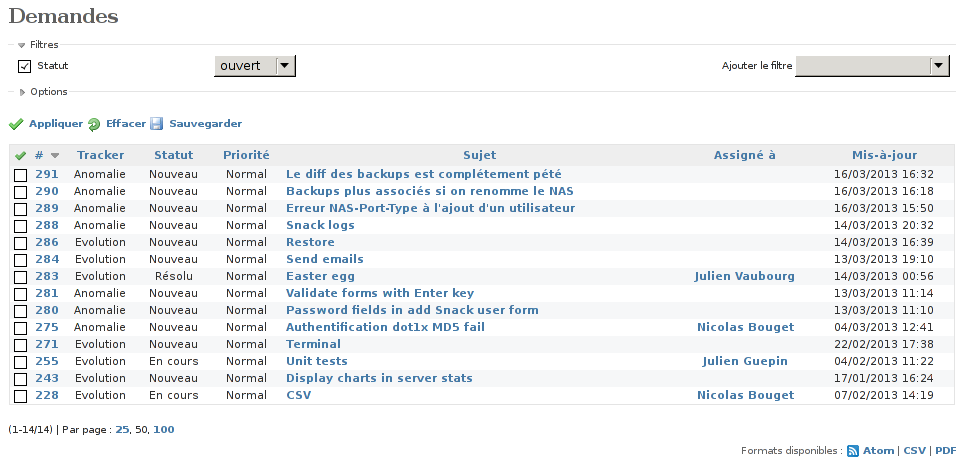
\includegraphics[width=0.9\textwidth]{img/tickets.png}
	\end{center}
	\caption{Gestionnaire de tickets.}
	\label{tickets}
\end{figure}

\subsubsection{Planning}

Un diagramme de Gantt des tâches prévues est disponible en annexe~\ref{gantt} page~\pageref{gantt}.

On y retrouve les deux principales étapes du projet, découpées en tâches, elles-même détaillées par des sous-tâches. Les principales tâches sont décrites dans la suite de ce document. La fin du travail sur les authentifications a eu lieu mi-novembre, et la fin de l'interface web liée aux fonctions du Radius mi-décembre. La fin de cette tâche marque la fin de la première grande étape du projet, qui est suivie par la seconde dès le début de l'année civile qui suit.

La liste des livrables proposée dans la note de cadrage (annexe~\ref{note-cadrage} page~\pageref{note-cadrage}) est la suivante~:

\begin{description}
\item[19 octobre 2012 :] Remise de la note de cadrage.
\item[5 novembre 2012 :] Signature de la note de cadrage.
\item[12 novembre 2012 :] Remise du cahier des charges.
\item[19 novembre 2012 :] Signature du cahier des charges.
\item[20 décembre 2012 :] Soutenance intermédiaire.
\item[7/8 février 2013 :] Audit du projet.
\item[14 mars 2013 :] Remise du projet avec les documentations.
\item[20 mars 2013 :] Remise du rapport.
\item[21 mars 2013 :] Soutenance finale.
\end{description}

\subsubsection{Attributions et réunions}

L'attribution des tâches aux membres du projet s'est faite sur la base du volontariat. Le groupe étant cohérent et dynamique, aucune tâche n'a été affectée de force. Cette méthode a fonctionné correctement tout au long du projet, permettant à chacun d'avancer sans contrariétés.

Une réunion de travail a été planifiée toutes les semaines, en présence de l'ensemble des membres de l'équipe et de l'intervenant industriel qui s'est montré disponible tout au long du projet. Une réunion mensuelle a eu lieu avec l'encadrant universitaire, lui permettant d'obtenir une interactivité régulière, complémentaire avec les rapports des réunions de travail reçus toutes les semaines.

\subsection{Documentation technique}

À mi-parcours du projet, l'entreprise nous a signifié que l'un de ses clients souhaitait utiliser notre travail en avant-première. L'interface n'était pas encore finie, et le paquet d'installation non-plus. Mais le client souhaitait une documentation technique, pour installer lui-même notre solution, en suivant nos recommandations.

Nous avons donc passé un temps non-négligeable à documenter toute la procédure d'installation manuelle de SNACK. Cette documentation est visible en annexe~\ref{doc-install} page~\pageref{doc-install}. Le client en question a salué la clareté de notre document.

\section{Choix effectués}
\subsection{Nom du projet}

Le nom du projet a été choisi par les étudiants. Il s'agit de \og~SNACK~\fg{} pour \og~\emph{Secure Network Access Control for Kids}~\fg.

Ce nom a été retenu pour ces quatre qualités~:

\begin{enumerate}
\item La signification de l'acronyme cadre parfaitement le but du projet, en évoquant le contrôle des accès du réseau.
\item Le \emph{for Kids} insiste sur l'objectif du projet, à savoir de proposer une solution clé-en-main.
\item L'acronyme fait référence à un autre mot anglais facile à retenir, ce qui est courant et apprécié dans les projets informatiques.
\item En plus de \emph{NAC}, l'acronyme a l'avantage de contenir le suffixe \emph{ACK} qui, à lui tout seul, évoque le réseau (les acquittements de TCP).
\end{enumerate}

Ce nom a été validé par l'encadrant industriel.

\subsection{Protocoles et implémentations}
\subsubsection{Contrôle des accès réseaux}

Lors des premières réunions avec l'intervant industriel, il a été convenu d'utiliser la technologie 802.1x pour répondre aux exigences du projet. Cette solution correspond particulièrement bien avec les objectifs, et est déjà connue au sein de l'entreprise.

Le 802.1x est un standard du réseau, largement utilisé dans les réseaux d'entreprise. Il s'agit d'un protocole implémenté au niveau des équipements actifs du réseau~: les commutateurs et les routeurs. Lorsqu'un poste client tente de se brancher physiquement à la prise murale de son bureau, celle-ci est désactivée par défaut. Une fois l'ordinateur relié, celui-ci prend connaissance de la présence de la technologie 802.1x sur le réseau, et interroge le commutateur auquel il accède. Pour ce faire, il lui envoie ce qui est nécessaire à son authentification. Selon le type d'authentification reconnu sur le réseau, il y a plusieurs possibilités~:

\begin{description}
\item[Par adresse MAC~:] Il s'agit de la méthode la plus simple à mettre en oeuvre, et à utiliser pour le poste client, puisqu'elle est totalement transparente. L'adresse MAC représente l'adresse physique de l'interface réseau du poste client, unique dans le monde. Elle suffit donc au commutateur, pour identifier celui qui tente de rejoindre le réseau, et l'autoriser ou non à y accéder. Le principal défaut de cette solution est qu'il est très facile d'usurper l'adresse d'un autre poste client, et de se faire passer pour lui, bénéficiant ainsi automatiquement de ses autorisations.
\item[Par mot de passe~:] En plus, ou non, de l'authentification par adresse MAC, l'authentification peut nécessiter un couple identifiant/mot de passe. Cette méthode résout le problème d'usurpation d'adresse, puisque le mot de passe assure qu'au moins une information est suffisamment secrète pour prévenir les vols d'identité. Le défaut majeur de cette possibilité est qu'elle n'est plus transparente pour l'utilisateur, qui devra saisir son identifiant et son mot de passe pour rejoindre le réseau. D'un point de vue de la sécurité, le mot de passe saisi transite en clair sur le réseau, permettant ainsi à un éventuel attaquant de le récupérer pour une future usurpation d'identité.
\item[Par certificat~:] Une dernière solution consiste à utiliser un système de certificats. Il en existe de plusieurs types, mais leur point commun à tous est de permettre aux postes clients de s'authentifier de façon totalement transparente, tout en assurant un chiffrement de la communication de bout en bout. Son défaut majeur, c'est que s'il est transparent à l'utilisation, il nécessite une première installation sur les postes clients concernés.
\end{description}

Après discussions entre membres de l'équipe sur les avantages et les inconvénients des différentes solutions, un exposé des problématiques a été présenté à l'intervenant industriel lors d'une réunion hebdomadaire. Chacune de ces solutions ayant ses avantages, l'intervenant a souhaité que toutes ces solutions soient implémentées dans la solution logicielle finale. Malgré sa faible fiabilité, l'authentification par adresses MAC est parfaitement adaptée aux périphériques comme les imprimantes. L'authentification par mot de passe est utile lorsqu'il s'agit de connexions ponctuelles d'utilisateurs invités. Quant à l'authentification par certificats, elle est nécessaire pour tous les permanents de l'entreprise qui bénéficient de permissions importantes sur le réseau.

Lorsque le poste client envoie les informations permettant son authentification au commutateur qui se situe à l'autre bout de la prise murale, ce dernier transmet automatiquement les informations à un serveur chargé de l'authentification et de la mise en place des autorisations. Si l'authentification est bonne, le serveur indique au commutateur l'action qu'il doit entreprendre dans le cadre du protocole 802.1x. Soit le port reste fermé, et le poste client n'a pas accès au réseau, soit il s'ouvre et le réseau est accessible. Selon le type d'utilisateur reconnu, le serveur peut spécifier un numéro de réseau virtuel (VLAN) en particulier. Cette spécificité aura pour effet de placer automatiquement le poste client dans un réseau qui bénéficie de plus ou moins de privilèges d'accès.

Le schéma~\ref{dot1x} page~\pageref{dot1x} résume le fonctionnement général du 802.1x. Le plus important à comprendre, c'est que le client (\emph{supplicant}) communique avec le commutateur (NAS) en EAP, et que ce dernier communique en conséquent avec le serveur d'authentification (le serveur SNACK) en RADIUS (la plupart du temps en encapsulant au passage le message EAP original). L'EAP est un protocole virtuel qui permet de s'abstraire des vrais protocoles utilisés, pour améliorer la compatibilité des commutateurs.

\begin{figure}[!h]
	\begin{center}
		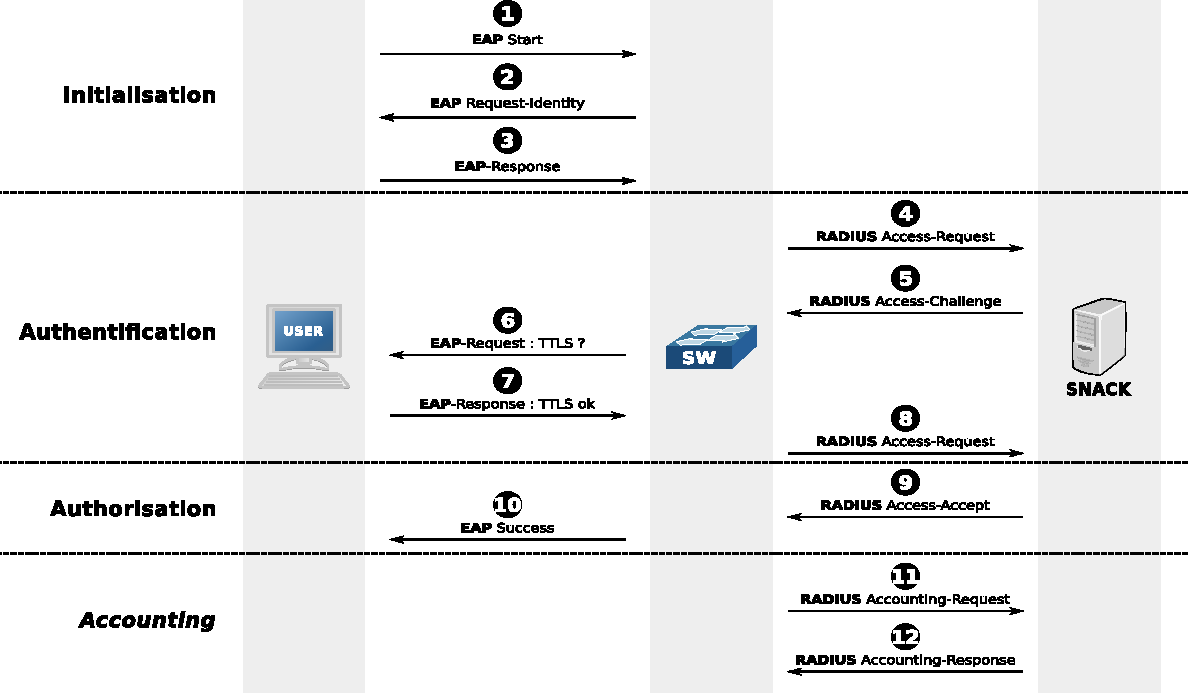
\includegraphics[width=0.9\textwidth]{img/dot1x-rapport.pdf}
	\end{center}
	\caption{Fonctionnement protocolaire du 802.1x.}
	\label{dot1x}
\end{figure}

Le serveur Radius est le seul à connaître la base des utilisateurs et les différents paramètres qui lui sont associés. Il s'agit d'un standard largement utilisé dans le cadre du 802.1x. Le client n'a aucune conscience de la présence du serveur Radius sur le réseau. Nous verrons plus en détail l'utilité de la dernière partie des échanges (\emph{accounting}) dans la section~\ref{accounting} page~\pageref{accounting}.

Cette technologie présente un second avantage pour l'entreprise~: en cas de remplacement du commutateur, la configuration du nouveau matériel sera rapide à remettre en place, dans la mesure où toutes les informations sont stockées au niveau du serveur d'authentification et les ports sont entièrement dynamiques.

Les serveurs d'authentification les plus connus dans le domaine des réseaux, et en particulier du 802.1x, sont ceux qui sont basés sur le protocole Radius. Il en existe plusieurs implémentations, parmi lesquelles un choix a dû être fait.

\subsubsection{Serveur d'authentification}

Le marché dispose de plusieurs dizaines d'implémentations différentes du protocole Radius. L'entreprise souhaitant se restreindre aux solutions libres, le choix se réduit automatiquement à une dizaine de solutions différentes.

Après avoir éliminé les implémentations trop anecdotiques, qui ne bénéficient ni d'un développement suivi ni d'une vraie communauté lui permettant d'assurer son avenir, trois implémentations ont été retenues~:

\begin{itemize}
\item FreeRadius
\item GnuRadius
\item OpenRadius
\end{itemize}

Ces trois solutions sont dominantes sur le marché des implémentations Radius Open Source.

L'étude destinée à les différencier pour n'en choisir qu'un seul a porté sur plusieurs critères~:

\begin{itemize}
\item Les fonctionnalités supportées.
\item La taille de la communauté et de la documentation.
\item La date de la dernière mise à jour du logiciel.
\end{itemize}

Sur la base de ces trois critères, FreeRadius est ressorti du lot. Outre ses fonctionnalités très complètes, le principal critère différenciateur fut le suivi du projet, avec une dernière mise à jour en 2012, contre 2008 pour GnuRadius et 2007 pour OpenRadius. Le projet FreeRadius bénéficie également d'une communauté exemplaire, et d'une documentation très fournie. Il s'agit d'une référence dans le monde de l'entreprise, et assure à B.H. Consulting un suivi du produit sérieux pour l'avenir. C'est également la seule solution qui dispose d'un paquet Debian/Ubuntu, facilitant d'autant plus son installation sur les serveurs.

\subsubsection{Types de certificats}

L'authentification des postes clients par certificats représente le moyen le plus simple et le plus sécurisé de se relier au réseau en utilisant la technologie 802.1x. Il existe plusieurs types d'authentification par certificats, qui apportent un niveau plus ou moins élevé de sécurité. Elles utilisent toutes le protocole EAP.

Protocoles d'authentification envisageables~:

\begin{description}
\item[TLS :] Il s'agit d'un protocole qui fonctionne par authentifications réciproques. Le client comme le serveur disposent de leur propre certificat, qu'ils commencent par s'échanger dans leur version publique. Chacun vérifie le certificat de l'autre, et un tunnel sécurisé peut être établi pour faire transiter les données, en ayant l'assurance que les deux protagonistes sont bien ceux qu'ils annoncent être. Un nom d'utilisateur peut être proposé par le client, qui fera l'objet d'une vérification par le serveur en fonction du champ \textit{CommonName} du certificat client utilisé.
\item[TTLS ou PEAP :] Ces deux protocoles sont relativement équivalents, avec une préférence pour le TTLS qui se repose sur des algorithmes plus sécurisés. La principale différence avec le TLS réside dans l'absence de certificat côté client, qui n'est donc pas identifié de façon fiable. Seul un couple utilisateur/mot de passe envoyé par ce dernier permet au serveur de l'identifier. Ces informations sont hashées (via MD5, pap, chap, mschap ou mschapv2) puis envoyées via le tunnel sécurisé. Ce passage est illustré par la figure~\ref{ttls} page~\pageref{ttls}.
\end{description}

\begin{figure}[!h]
	\begin{center}
		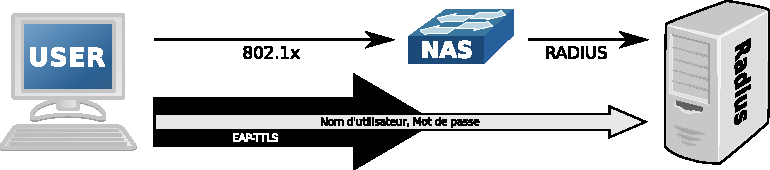
\includegraphics[width=0.7\textwidth]{img/ttls.pdf}
	\end{center}
	\caption{Passage des informations d'authentification en TTLS (double-chiffrement)}
	\label{ttls}
\end{figure}

Dans les trois cas, le serveur dispose d'un  certificat d'autorité qu'il a lui-même généré, en version privée comme publique. Il dispose également d'un certificat d'authentification qu'il a pris soin de s'auto-signer. Les clients ont accès à la version publique de ce dernier. Avec la version publique du certificat d'autorité, ils vérifient la validité du certificat d'authentification publique diffusé par le serveur.

Dans le cas du TLS, le client s'est fait délivrer un couple de certificats privé/publique par le serveur, signés par ce dernier avec le certiticat d'autorité.

En accord avec l'intervenant industriel, nous sommes arrivés à la conclusion qu'il fallait que les authentifications proposent le TLS et le TTLS, pour offrir le choix aux entreprises. Concernant le chiffrement des informations transmises dans le tunnel dans le cas du TTLS, les recherches effectuées aboutissent à la conclusion que la solution mschapv2 est la plus sécurisée. Elle devra donc être utilisée en priorité par les clients.

\subsection{Interface web}
\subsubsection{Langages et environnements de développement}

Le langage PHP a été imposé pour la conception de l'interface web du projet. Le langage a l'avantage d'être suffisamment populaire chez les développeurs, pour assurer sa maintenabilité dans le futur. Il permet une approche de la conception propre et cohérente avec les techniques de développement actuelles, en offrant des performances acceptables y compris pour des serveurs de faible capacité.

Une contrainte sur l'environnement de développement est rapidement venue s'ajouter au langage imposé. Les développeurs de B.H. Consulting ont demandé que l'interface exploite les possibilités du \textit{framework} Bootstrap Twitter. Ce dernier est particulièrement populaire depuis sa récente création par l'entreprise du même nom. Il s'agit d'un composant logiciel pour la partie cliente de l'interface, qui propose une collection très complète de feuilles de style et de dispositions pour créer les vues, afin d'offrir une expérience utilisateur confortable. Une formation rapide de cet outil en interne a dû être effectuée par les membres de l'équipe qui ne l'avaient jamais utilisé auparavant.

Du côté du serveur, l'utilisation d'un \textit{framework} est également conseillée, pour forcer une programmation cohérente et organisée de façon stricte. Il existe plusieurs solutions sur le marché, qui ont conduit à une étude au sein de l'équipe de la meilleure solution à proposer pour la réalisation du projet.

Les plus populaires et puissantes qui ont été retenues sont~:

\begin{itemize}
\item CakePHP
\item CodeIgniter
\item Symfony
\item Yii
\item Zend Framework
\end{itemize}

La conclusion de l'étude a poussé l'équipe à se tourner vers la solution CakePHP. Il s'agit en effet d'un des premiers outils de ce type a être développé pour PHP, basé sur la réalisation de Ruby On Rails, le premier du genre. Il bénéficie donc d'une maturité exemplaire, et dispose d'une communauté rassurante, avec une documentation très complète et très détaillée. La prise en main du logiciel est particulièrement rapide, tout en laissant une grande liberté d'adaptation à tous les usages.

CakePHP n'offre pas toutes les possibilités avancées disponibles avec des solutions plus importantes comme Zend Framework ou Symphony, comme les bibliothèques d'interaction avec d'autres services web tiers (comme Google), mais les fonctionnalités fournies suffisent largement pour le projet et les évolutions qu'il pourrait raisonnablement connaître. Les performances sont particulièrement bonnes en comparaison à ses concurrents plus complets. La solution Yii aurait permis de construire une application qui tient un peu mieux la charge avec des milliers d'utilisateurs, mais l'usage auquel il est destiné pour le projet ne nécessite pas de prendre en compte de telles problématiques.

CakePHP est disponible sous licence libre (MIT). Les patrons de conception populaires sont disponibles, comme le MVC (modèle-vue-contrôleur) qui permet de segmenter l'application de façon propre et efficace. Un fonctionnement en \textit{ActiveRecord} est également disponible, permettant à des classes PHP d'abstraire totalement la liaison entre l'application et la base de données. Les méthodes du modèle intégrent les opérations CRUD (\textit{create}, \textit{read}, \textit{update}, \textit{delete}) permettant de développer rapidement. De nombreuses autres fonctionnalités sont disponibles, comme un dispacheur d'URL, la validation des données, le moteur de patrons facilitant le formatage, la gestion d'un cache, des composants de sécurité et des scripts de génération de code.

La proposition à l'intervenant industriel de cette solution a particulièrement bien été accueillie puisqu'un développeur de l'entreprise utilise cette solution régulièrement, et sera donc à même de maintenir l'interface dans le futur.

\subsubsection{Gestionnaire de bases de données}

Entre les solutions basées sur des implémentations SQL et les nouvelles possibilité de NoSQL (solution alternative qui consiste à ne pas systématiquement privilégier le modèle relationnel), le choix est vaste pour stocker les informations liées à l'interface. Une solution libre étant demandée par l'entreprise, quelques solutions ne sont dors et déjà pas envisageables. 

La meilleure solution pour faire interagir l'interface web avec le serveur Radius étant de réussir à faire fonctionner ce dernier avec une base de données plutôt qu'une collection de fichiers, le choix de la solution s'est fait en ne gardant que les solutions supportées par le fonctionnement de FreeRadius (l'implémentation de Radius choisie auparavant). Cette contrainte élimine toutes les solutions de NoSQL, et réduit le choix aux solutions populaires MySQL et PostgreSQL, éliminant des solutions plus légères comme SQLite qui auraient pu convenir.

PostgreSQL est beaucoup plus puissant que MySQL, mais il est aussi beaucoup plus lourd et plus contraignant à mettre en place. Les possibilités offertes par MySQL et sa simplicité conviennent parfaitement aux exigences du projet.

Le choix de cette solution a été accueilli favorablement par l'intervenant industriel.

\subsubsection{Journaux systèmes}

Pour une meilleure traçabilité des actions des clients, l'interface web doit impérativement enregistrer les actions qu'elle effectue. Elle doit également être capable de présenter les journaux du Freeradius, de façon conviviale.

Nous avons choisi d'utiliser le logiciel Syslog-ng couplé à une base de données MySQL pour la gestion de ces derniers. Ainsi, le Freeradius écrit directement, via Syslog-ng, dans la base de données que l'interface peut alors exploiter. Nous avons également conçu l'interface de telle sorte que toutes les traces que nous générons soient stockés dans cette même table avec un indicateur différent.

Ainsi, la gestion des journaux systèmes des différents composants est homogène et se fait à l'aide d'un outil largement répandu, qui permettra de facilement ajouter des onglets pour afficher d'autres types de journaux.

\subsubsection{Internationalisation}

Pour permettre à notre travail d'être éventuellement réexploitable au delà des frontières franco-luxembourgeoises, l'interface a été écrite en anglais. Nous avons ensuite utilisé un outil nous permettant de traduire l'interface à la main en français. Ainsi, à n'importe quel instant, l'utilisateur a la possibilité de passer l'interface entièrement en anglais ou en français. L'intégration d'une nouvelle langue se fera très aisément, simplement en ajoutant les fichiers de langue correspondants.

La langue par défaut dépendra de la localisation du visiteur, c'est à dire de la langue de son navigateur.

\subsection{Sauvegarde des configurations}
\label{chap-sauvegardes}
\subsubsection{Rêve d'administrateur}

Imaginez un monde où le risque zéro existe, où n'importe quel administrateur réseau peut se permettre de modifier la configuration de ses équipements sans se préoccuper de la sauvegarde de la configuration initiale. Un monde sans risque qui interdit aux débutants de faire l'erreur qui leur coûtera une longue soirée à retrouver les choix effectués avant qu'il ne se lance dans des changements hasardeux qu'il aura finalement abandonnés. En somme un monde où le prestataire du réseau est assuré qu'il n'aura jamais à refaire deux fois le même travail, par sa faute ou par la faute de son client. C'est le défi qui nous a été imposé par B.H. Consulting, qui trouve un intérêt particulièrement grand dans cette vision idéaliste.

Le concept est simple~: chaque fois qu'un administrateur se connecte sur un équipement réseau, la configuration de ce dernier devra être sauvegardée sur un serveur centralisé. Elle le sera également lorsqu'il se déconnecte, et lorsqu'il enregistre ses modifications sur le disque de l'équipement. Ainsi, aucune modification ne pourra être oubliée, et l'historique est intégralement sauvegardé pour lui permettre de revenir en arrière aisément.

Pour répondre à cette demande, notre équipe a dû redoubler de travail afin de trouver les solutions adéquates pour détecter l'un de ces trois événements, déclencheurs d'un rappatriement immédiat des configurations.

\subsubsection{Sauvegarde de la configuration}

Sur un équipement Cisco, la configuration qui est utilisée est stockée dans la \emph{running-configuration}, elle-même stockée dans la mémoire vive. Cette dernière étant réinitialisée à chaque redémarrage, une modification durable (\emph{write memory}) doit donner lieu à une synchronisation entre la \emph{running-configuration} et la \emph{startup-configuration}. Cette dernière sera chargée au démarrage pour devenir la \emph{running} actuelle. 

La synchronisation entre la \emph{running-configuration} et la \emph{startup-configuration} sur le commutateur est une action à la discrétion de l'administrateur, totalement décorellée de l'\emph{accounting}. Pour lancer une sauvegarde automatique lors de cette action, il faut alors détecter un événement asynchrone et imprévisible.

Nous avons donc dû recourir au protocole SNMP. Ce dernier est particulièrement utilisé dans la supervision des réseaux, et propose une interface de communication épurée et facile à prendre en main. Ses messages sont systématiquement de type \og~OID~: valeur~\fg, que ça soit pour une question ou une réponse. Puisque c'est un standard largement utilisé, tous les équipements Cisco implémentent des fonctionnalités l'exploitant. Ainsi, dès lors que le commutateur est correctement configuré, un événement SNMP est envoyé à chaque enregistrement de la configuration. Un serveur externe peut alors attraper ce message (on parle de \emph{trap} dans le vocabulaire SNMP), en déduit l'action effectuée en fonction de l'OID (l'identifiant unique d'une ressource particulière) et de sa valeur, et exécute le script correspondant.

Le schéma~\ref{schema_wrmem} page~\pageref{schema_wrmem} illustre le mécanisme que nous avons mis en place pour exploiter cette possibilité. Un gestionnaire de versions est utilisé pour stocker les configurations de chacun des commutateurs, ce qui permet de les stocker de façon incrémentale, c'est à dire en ne stockant que les changements (\emph{commits}).

\begin{figure}[!h]
	\begin{center}
	    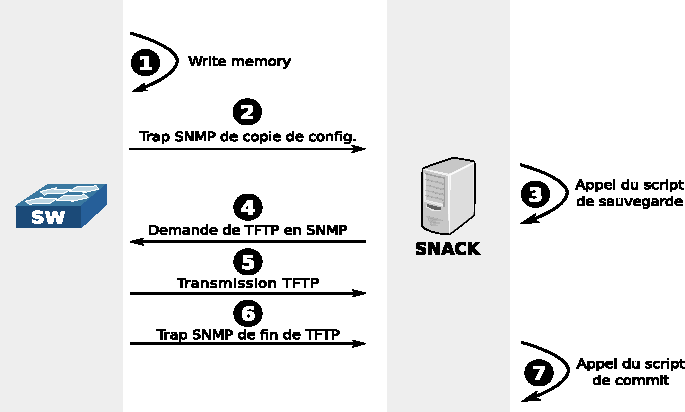
\includegraphics[width=0.7\textwidth]{img/wrmem.pdf}
	\end{center}
	\caption{Interactions entre le commutateur et le serveur SNACK lors d'une synchronisation (\emph{Write memory}).}
	\label{schema_wrmem}
\end{figure}

À noter que les matériels Cisco ne permettent de récupérer leur configuration qu'au travers du protocole TFTP. Celui-ci est une version simplifiée du protocole de transfert de fichiers FTP, non-sécurisée. Toutefois, les transferts devraient avoir lieu dans un réseau virtuel suffisamment restreint pour que ça ne puisse pas poser de problème.

Un autre problème de taille de ce protocole imposé, est qu'il n'est pas orienté connexion. Ainsi, il est impossible de détecter la fin d'un transfert, pour l'ajouter ensuite dans le gestionnaire de versions. C'est pour cette raison que le schéma~\ref{schema_wrmem} page~\pageref{schema_wrmem} montre l'utilisation d'une nouvelle trap SNMP, que nous avons découverte, pour détecter la fin de l'opération.

Les deux autres événements sont plus simples à détecter, grâce à l'\emph{accounting}.

\subsubsection{Détection des connexions / déconnexions}
\label{accounting}

Une partie de l'équipe ayant travaillé sur le module de gestion des sessions, une bonne partie du travail a déjà été effectuée pour comprendre les mécanismes d'\emph{accounting} de Freeradius. Cette fonctionnalité est utilisée en général pour identifier la longueur d'une session, dans le but de la facturer. Elle assure donc de correctement détecter son début et sa fin. Après différents tests, nous avons constaté que la fin de session intervenait quoiqu'il arrive, au pire grâce à un délai d'expiration. La seule exception étant une coupure électrique brutale du commutateur, pour laquelle nous avons mis en place un mécanisme de détection du démarrage permettant de fermer automatiquement toutes les sessions résiduelles restées ouvertes.

Nous avons choisi de créer un module Freeradius, qui est appellé à chaque événement de l'\emph{accounting}. Une condition filtre directement ces événements pour éliminer tout ce qui relatif aux connexions 802.1x, en se contentant de repérer les connexions/déconnexions sur le commutateur, en Telnet, SSH comme en série.

Le schéma~\ref{schema_auth} page~\pageref{schema_auth} illustre les interactions entre l'administrateur, le commutateur et le serveur SNACK lorsqu'une connexion Telnet, SSH ou série a lieu. Le processus est identique lorsqu'il se déconnecte.

\begin{figure}[!h]
	\begin{center}
	    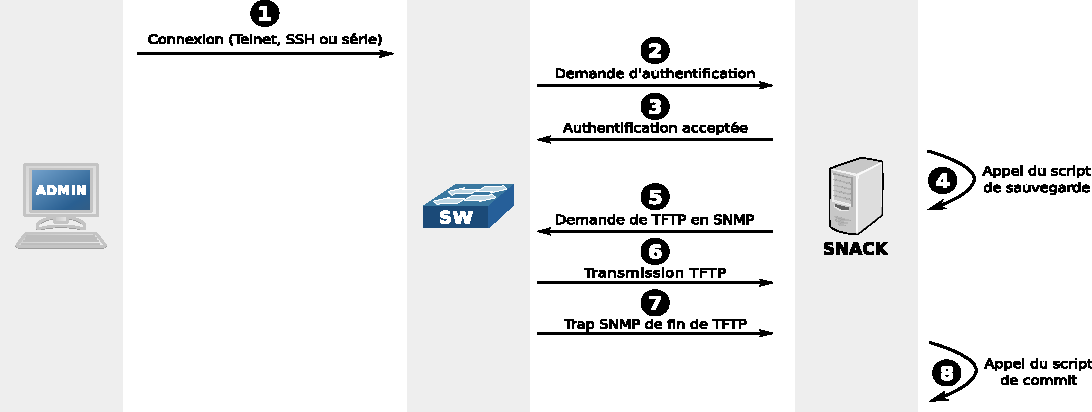
\includegraphics[width=\textwidth]{img/auth.pdf}
	\end{center}
	\caption{Interactions entre les différents composants lors d'une connexion Telnet/SSH/série.}
	\label{schema_auth}
\end{figure}

La principale différence avec le schéma précédent est que le processus de sauvegarde est déclenché automatiquement par l'utilisateur, directement depuis le serveur SNACK, plutôt qu'indirectement par le commutateur.

\subsection{Installation automatisée}

Pour que notre solution logicielle soit facilement et rapidement déployable sur de nombreux parcs informatiques, nous avons choisi de profiter de la puissance du gestionnaire de paquets du système cible. Ainsi, nous avons conçu un simple paquet Debian, qui s'occupe d'installer tous les fichiers et toutes les dépendances, pour une solution entièrement clé en main.

Pour plus de confort, le paquet propose une interface d'installation conviviale, comme l'illustrent les copies d'écran en figure~\ref{install_start} page ~\pageref{install_start}, \ref{install_prompt} page \pageref{install_prompt} et \ref{install_progress} page \pageref{install_progress}.

\begin{figure}[!h]
	\begin{center}
	    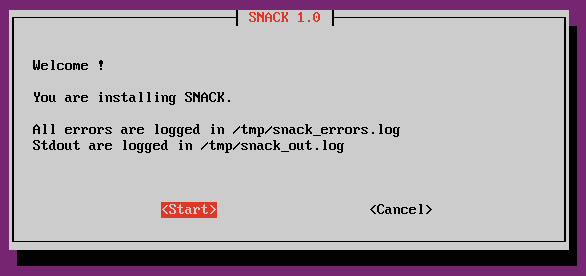
\includegraphics[width=0.6\textwidth]{img/install_start.png}
	\end{center}
	\caption{Accueil de l'installation du paquet SNACK.}
	\label{install_start}
\end{figure}

\begin{figure}[!h]
	\begin{center}
	    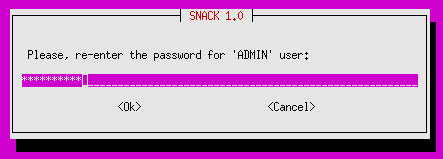
\includegraphics[width=0.6\textwidth]{img/install_prompt.png}
	\end{center}
	\caption{Exemple d'invite de saisie lors de l'installation du paquet SNACK.}
	\label{install_prompt}
\end{figure}

\begin{figure}[!h]
	\begin{center}
	    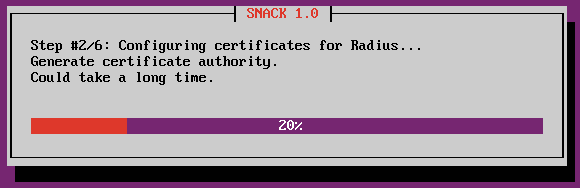
\includegraphics[width=0.6\textwidth]{img/install_progress.png}
	\end{center}
	\caption{Barre de progression pour une meilleure expérience utilisateur.}
	\label{install_progress}
\end{figure}

Une fois le paquet installé et les quelques questions répondues, le serveur est entièrement opérationnel et l'interface web immédiatement accessible (avec pour seul utilisateur, le super-utilisateur créé durant l'installation).

\section{Implémentations et méthodologies}
\subsection{Radius}

L'étude des différentes solutions radius aura occupé quelques jours du début du projet, comme en atteste la tâche issue du diagramme de Gantt disponible en figure~\ref{gantt_radius} page~\pageref{gantt_radius}.

\begin{figure}[!h]
	\begin{center}
		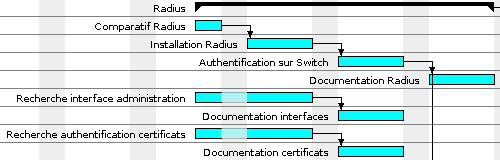
\includegraphics[width=350pt]{img/gantt_radius.png}
	\end{center}
	\caption{Tâche \textit{Radius}}
	\label{gantt_radius}
\end{figure}

Elle a commencé par une recherche documentaire généraliste sur le protocole Radius pour tous les membres de l'équipe, qui a abouti sur l'écriture d'une courte documentation interne. S'en est suivi une recherche plus précise sur les différentes implémentations existantes. Une fois la liste établie, chaque membre a pu s'intéresser plus particulièrement à une solution précise.

La liste des avantages et des inconvénients de chacun a été dressée en réunion, pour conclure sur l'implémentation la plus adaptée à proposer à l'intervenant industriel.

\subsection{Bases de données SQL}

Les recherches concernant le choix de la solution de gestion de bases de données est intimement liée à celui de l'implémentation radius. Ces deux tâches ont donc été exécutées en parallèle, pour trouver une solution globale dans laquelle tous les éléments savent interagir ensemble, tout en étant la plus performante possible.

Le détail de cette tâche issu du diagramme de Gantt est donné en figure~\ref{gantt_sql} page~\pageref{gantt_sql}.

\begin{figure}[!h]
	\begin{center}
		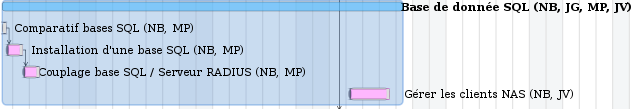
\includegraphics[width=350pt]{img/gantt_sql.png}
	\end{center}
	\caption{Tâche \textit{Bases de données SQL}}
	\label{gantt_sql}
\end{figure}

Après avoir dressé une liste des solutions Open Source les plus populaires, une recherche documentaire a été effectuée sur chacune, pour prendre en compte ses avantages et ses inconvénients. La compatibilité avec les trois principales implémentations Radius retenues a aussi été un critère de choix.

La solution retenue a été installée sur une machine de tests, au côté du Radius gagnant. Une dernière étape a consisté à réussir à lier les deux, pour que l'authentification Radius utilise la base de données SQL.

\subsection{802.1x}

Une dernière étape demeure dans le domaine de la base de données~: gérer les clients NAS, c'est à dire les commutateurs qui auront à utiliser le Radius (et donc indirectement la base de données).

Cette étape s'est faite en parallèle de l'étude du protocole 802.1x, décrite dans la figure~\ref{gantt_dot1x} page~\pageref{gantt_dot1x}.

\begin{figure}[!h]
	\begin{center}
		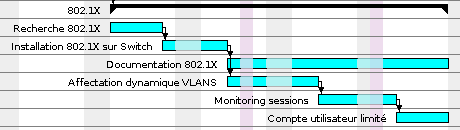
\includegraphics[width=350pt]{img/gantt_dot1x.png}
	\end{center}
	\caption{Tâche \textit{802.1x}}
	\label{gantt_dot1x}
\end{figure}

Celle-ci a logiquement commencé par l'écriture d'une documentation sur le standard, qui a permise à l'équipe de s'auto-former sur la technologie. Après avoir réussi à appliquer nos connaissances sur un commutateur, l'affectation dynamique de réseau virtuel a été testée. Cette première étape valide le coeur-même de notre projet, qui consiste à permettre à une entreprise de graviter le plus simplement possible autour de cette possibilité.

Diverses autres possibilités ont été testées à la main, pour comprendre ce que le protocole permet effectivement de faire, et qui peut nous être utile pour l'implémentation de l'interface web en vue de répondre aux exigences demandées. Ainsi, les tests sur la supervision des sessions ont permis de cerner les différentes possibilités pour identifier le début et la fin d'une session, qui pourra ensuite être affichée graphiquement dans l'interface web. D'autres études comme les limitations pour un utilisateur et les journaux systèmes préparent les futures fonctionnalités de l'interface.

\subsection{Authentifications}

Étape critique du projet, les authentifications au travers du Radius ont été essentielles pour présager du bon fonctionnement de l'ensemble du projet. Elle est décrite dans la figure~\ref{gantt_auth} page~\pageref{gantt_auth}.

\begin{figure}[!h]
	\begin{center}
		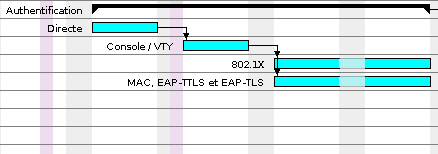
\includegraphics[width=350pt]{img/gantt_auth.png}
	\end{center}
	\caption{Tâche \textit{Authentifications}}
	\label{gantt_auth}
\end{figure}

Les premiers tests ont concerné le Radius directement, et ont abouti sur une authentification de client Radius sur un serveur Radius réussie. La suite aura concerné les commutateurs directement, sur lesquels l'authentification peut se faire aussi directement en Radius (accès à l'interface de configuration du système). Les tests étant concluants, il est possible de contrôler les accès à la configuration d'un commutateur directement grâce à Radius, aussi bien via telnet que le port console.

La suite logique a été de tester directement le protocole 802.1x. L'authentification d'un client sur le Radius au travers du commutateur fonctionnant, il ne reste plus qu'à décliner les solutions pour la certifier.

Jusqu'alors, les authentifications ont été faites en MD5, c'est-à-dire avec uniquement un couple utilisateur/mot de passe, simplement chiffré sur le réseau. Beaucoup de solutions existent, offrant des possibilités très diverses en terme de sécurité et de simplicité d'utilisation. Ces solutions ont été étudiées, documentées, testées et enfin élaguées.

\subsection{Procédure d'installation}

Une fois les différentes tâches concernant le Radius et le SQL terminées, une réinstallation totale du système a été effectuée. Il a ensuite été réinstallé pas-à-pas, grâce aux documentations réalisées durant les tests. Cette étape a été l'occasion de corriger la documentation, et de se confronter à d'autres problèmes mineurs. Cette tâche est décrite en figure~\ref{gantt_finalisation} page~\pageref{gantt_finalisation}.

\begin{figure}[!h]
	\begin{center}
		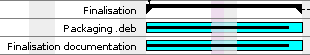
\includegraphics[width=0.5\textwidth]{img/gantt_finalisation.png}
	\end{center}
	\caption{Tâche \textit{Finalisation}}
	\label{gantt_finalisation}
\end{figure}

Un paquet Ubuntu a été réalisé au fur et à mesure de la réinstallation, pour permettre son automatisation. Une dernière réinstallation aura permis de tester son bon fonctionnement. Ce paquet permettra un gain de temps précieux pour l'entreprise, qui aura à le déployer sur toutes les machines d'authentification de ses clients. Différentes questions sont posées durant son installation, pour qu'il s'adapte le plus simplement possible au client.

La réinstallation du système a posé plusieurs fois problème~: les machines mises à disposition ne sont pas parfaitement supportées par Ubuntu et Windows XP. Beaucoup de temps a été perdu pour résoudre les différents problèmes rencontrés.

\subsection{Radius par le web}

Le projet arrivant à maturité pour ses fondements internes, l'accent a été mis sur la conception de l'interface web, permettant de contrôler ce qui a été réalisé d'une façon simple, ergonomique et conviviale. Cette tâche est racontée en figure~\ref{gantt_cake} page~\pageref{gantt_cake}.

\begin{figure}[!h]
	\begin{center}
		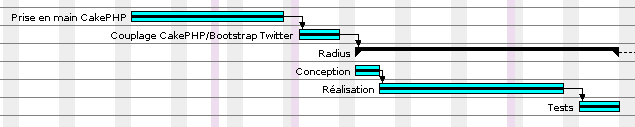
\includegraphics[width=0.8\textwidth]{img/gantt_cake.png}
	\end{center}
	\caption{Tâche \textit{Interface web}}
	\label{gantt_cake}
\end{figure}

La première grosse partie a été de créer une interface pour le Freeradius. Il en existe beaucoup de disponibles, mais aucune n'est satisfaisante, ce qui a rendu le défi d'autant plus intéressant. Cette tâche a nécessité de comprendre parfaitement les mécanismes internes de ce que nous avions mis en place, pour l'ensemble des membres de l'équipe. C'est ainsi que sont nées la gestion des utilisateurs, des groupes, des commutateurs, des sessions et des journaux systèmes.

L'association de Bootstrap Twitter avec CakePHP n'a pas été simple, et nous a demandé beaucoup de travail d'intégration. Autant que faire ce peut, nous avons apprivoisé les \emph{Components}, \emph{Elements} et autres facilités de CakePHP pour créer des modules réexploitables partout dans l'interface.

\subsection{Le module de sauvegardes}

Après un court passage par l'internationalisation (qui nous aura value ensuite plusieurs séances de traduction), la tâche visible en figure~\ref{gantt_sauvegardes} page~\pageref{gantt_sauvegardes} a annoncé le début d'une nouvelle étape~: le module de sauvegardes.

\begin{figure}[!h]
	\begin{center}
		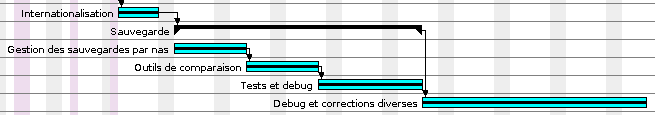
\includegraphics[width=0.8\textwidth]{img/gantt_sauvegarde.png}
	\end{center}
	\caption{Tâche \textit{Sauvegardes}}
	\label{gantt_sauvegardes}
\end{figure}

Ce nouveau défi nous a value de revenir à la configuration de Radius, Cisco, et cie. Grâce à des astuces qui sont décrites dans la section~\ref{chap-sauvegardes} page~\pageref{chap-sauvegardes}, nous sommes parvenus à récupérer les sauvegardes au moments clés que l'entreprise souhaitait. Il a fallu ensuite revenir sur CakePHP, pour développer la partie de l'interface qui lui est dédiée. Ainsi, toutes les sauvegardes sont visibles en temps réel sur l'interface, et peuvent être comparées graphiquement.

Cette tâche a eu lieu en parallèle de l'intégration de l'interface dans le paquet, et de la correction de problèmes détectés dans la partie précédente.

\subsection{La tâche qui n'aura pas lieu}

Le projet initial était très ambitieux, tant bien que nous avons finalement décidés d'abandonner la tâche qui avait été jugée la moins urgente par l'entreprise. Ainsi, la création d'un terminal virtuel, destiné à pouvoir contrôler les commutateurs depuis l'interface web sans avoir à demander d'accès au client, en restera à une démonstration minimale qui n'a rien d'exploitable. La défunte tâche est présentée en figure~\ref{gantt_terminal} page~\pageref{gantt_terminal}.

\begin{figure}[!h]
	\begin{center}
		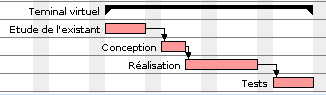
\includegraphics[width=0.5\textwidth]{img/gantt_terminal.png}
	\end{center}
	\caption{Tâche \textit{Terminal virtuel}}
	\label{gantt_terminal}
\end{figure}

Le temps récupéré suite à cette décision nous a permis de poursuivre les tests des autres parties, et de peaufiner l'interface pour la rendre encore plus conviviale. Nous avons en outre estimé que la création complète propre et sérieuse d'un terminal virtuel aurait pu donner lieu à un projet à part entière.

\subsection{Difficultés rencontrées}

Comme dans tout projet, de nombreux problèmes ont dû être surmontés. Voici la liste des principaux qui ont retenu notre attention~:

\begin{description}
\item[Matériel à disposition] Le projet a relativement mal commencé à cause du matériel qui a été mis à notre disposition. Sur les deux ordinateurs, l'un refusait d'installer Windows XP (disque dur soit-disant corrompu), et l'autre posait de gros problèmes avec Ubuntu (la carte graphique étant en cause, y compris en TTY). À noter aussi le lecteur CD-ROM cassé, et les adresses IP statiques qui nous ont été attribuées qui n'ont pas été sorties de l'intervalle IP du DHCP (entraînant régulièrement des déconnexions à cause de \og~vols d'IP~\fg{} involontaires de la part des autres utilisateurs). Nous sommes finalement arrivés à bout du problème de Ubuntu, nous avons emprunté un autre ordinateur pour le Windows, et nous avons installé un routeur avec notre propre NAT pour ne plus être ennuyé par les vols d'adresses (en privilégiant, dans une moindre mesure, l'utilisation des IPv6).
\item[VM-Project] Le gestionnaire de projet imposé par l'École aura été très laborieux à ses débuts. Nous avons pris le temps de remonter de nombreux bugs à l'éditeur, et nous avons eu à plusieurs reprises des pertes de feuilles de temps ou de rapports, pourtant très longs à ajouter.
\item[CakePHP avec Bootstrap] Le projet CakePHP propose son propre environnement graphique, et n'a pas été prévu pour être couplé avec Bootstrap Twitter. Pour se conformer à la demande de l'entreprise, nous avons progressivement écrit un script permettant de faire l'intégration le plus proprement possible, ralentissant d'autant notre écriture de l'interface.
\item[Schémas Radius avec CakePHP] Les modèles de CakePHP sont très puissants, et permettent de gagner beaucoup de temps. Mais il nécessite une base de données classique, ce qui n'est pas le cas de la table imposée par Freeradius. Ce dernier s'étant contenté de retranscrire ses fichiers de configuration texte en base de données, le domptage de CakePHP pour cette structure fut très laborieux. Nous avons finalement réussi à réutiliser la base de données, au prix de quelques fonctionnalités avancées qui ne peuvent plus être exploitées.
\item[Radius avec Cisco] Si la documentation de Freeradius est bien fournie, c'est moins vrai pour les interactions entre les commutateurs Cisco et le Radius. Nous avons dû prendre beaucoup de temps pour observer nous-mêmes certains échanges réseaux, parfois très complexes.
\item[MIB Cisco] L'utilisation de SNMP a demandé de parfaitement comprendre de quelle façon Cisco gère ses OID, pour déterminer quel numéro pour quelle valeur doivent être attendus pour un événement particulier. La documentation Cisco étant très évasive sur ce sujet, notre bonne compréhension a nécessité beaucoup de tests et d'observation de ses comportements.
\item[Versions Cisco] Les deux problèmes cités ci-dessous sont accentués par une compatibilité rarement assurée d'une version à l'autre par Cisco. Ainsi, certaines commandes ne sont plus valides d'un IOS à l'autre, lorsque ça n'est pas les valeurs par défaut qui changent. Difficile dans ce contexte de proposer des commandes automatisées ou de faire des documentations qui soient systématiquement valables. Après s'être bien documentés, nous avons tenté d'utiliser les solutions qui couvraient un maximum de matériels différents.
\item[Utilisation du TFTP] Les transferts de configuration Cisco ne peuvent se faire qu'en TFTP. Nous n'avons donc pas trouvé de solution pour les sécuriser, sur les commutateurs qui ne proposent pas de SSH. Puisqu'il s'agit d'un protocole sur UDP, nous n'avons pas non plus eu la possibilité d'exploiter un marqueur de fin de transfert, nécessaire pour exécuter nos scripts. Nous avons donc dû trouver des solutions annexes pour dépasser ce genre de contraintes.
\item[Certificats Windows] Après avoir réussi à gérer tous les types de certificats sous GNU/Linux, nous avons eu la mauvaise surprise de constater qu'ils ne fonctionnaient pas sous Windows. Nous avons été contraints de revenir en arrière, pour trouver un format unique qui soit compatible aussi bien sous Windows XP que GNU/Linux. C'est le format PEM qui a le mieux convenu, mais celui-ci contient à la fois la clé privée et la clé publique. Ce qui est pratique pour les certificats clients, mais inutilisable pour les certificats serveurs (dont on ne distribue que la version publique). Il faut donc utiliser un chemin détourné sous Windows XP pour l'installer, plutôt que de simplement double-cliquer sur l'icône du fichier.
\item[Fichiers des paquets] L'installation du serveur est gérée directement par le gestionnaire de paquets de Ubuntu, grâce à notre paquet de type Debian. S'il n'y a aucun problème à déployer des fichiers de cette façon, c'est beaucoup plus compliqué lorsque l'on souhaite adapter la configuration d'autres paquets (comme Freeradius, par exemple). Pour éviter les conflits, nous avons dû lancer des commandes de modification des fichiers de configuration dans le script de post-installation. La principale conséquence de cette technique, qui fonctionne très bien, c'est qu'il est impossible de désinstaller le paquet en enlevant l'intégralité de ses traces. Heureusement, de plus en plus de logiciels intégrent un système de configuration décomposable dans un dossier de type \emph{config.d}.
\item[Tests du paquet] Tester l'installation du paquet a nécessité de repartir systématiquement d'un système d'exploitation vierge. Une collection de machines virtuelle a dû être mise en place à cet effet, nécessitant d'attendre chaque fois leur redémarrage.
\item[Navigateurs] La compatibilité de l'interface avec les différentes versions des navigateurs a été très contraignante à surveiller, notamment à cause de Internet Explorer qui nécessite de lancer un Windows, que personne n'utilise au quotidien.
\item[Fichiers de langue] L'internationalisation de l'interface a été gérée proprement avec des fichiers de langue. Ces derniers sont éditables via un logiciel standard, permettant de traduire toutes les chaînes de caractères que CakePHP a automatiquement extraits. Nous avons constaté à nos dépends que les traductions ne sont pas toujours possibles, sans connaître le contexte exact de la chaîne de caractères. Il nous aura fallu de nombreux passages sur les fichiers de langues pour que l'interface soit cohérente en anglais (langue par défaut) comme en français.
\end{description}

Dans l'ensemble, si un temps excessif a parfois été perdu pour corriger des problèmes délicats, ils ont tous été surmontés ou contournés. Malgré tout, le temps perdu a modifié notre planning et nous a contraint à renoncer à la dernière tâche, le terminal virtuel.

\section{L'interface web}
\subsection{L'administration à la portée de tous}

Les employés de B.H. Consulting en majorité de valeureux et talentueux administrateurs systèmes. La ligne de commandes est à leur portée, et les interfaces austères (et néammoins très efficaces) ne les rebutent pas. Mais ce qui est vrai en interne ne l'est pas forcément en externe. Ainsi, les clients qui sont les leurs n'ont pas systématiquement les compétences pour administrer leurs réseaux sans être guidés, et sans une nécessité certaine de mise en confiance par l'outil. Une interface graphique, colorée et assurément ergonomique est un luxe que B.H. Consulting souhaite leur apporter. L'outil le plus simple pour contacter une application étant le navigateur web, c'est le choix que nous avons fait.

Une grosse partie de notre travail a donc consistée à dissimuler les mécanismes complexes que nous avons mis en place, derrière un outil accessible. Puisque les outils mis en oeuvre ont déjà été présentés dans une autre section, celle-ci est dédié à la présentation de l'aboutissement de notre projet, et de ses choix ergonomiques. Puisque ce sera probablement la langue la plus exploitée, l'interface est présentée en français.

\subsection{Vue générale}

L'accueil sur l'interface se fait avec une invitation à s'identifier (figure~\ref{login} page~\pageref{login}). Il faut être un utilisateur SNACK enregistré pour pouvoir y accéder, complétement ou partiellement. La création d'un utilisateur ayant tous les droits dessus est demandée lors de l'installation du paquet.

\begin{figure}[!h]
	\begin{center}
	    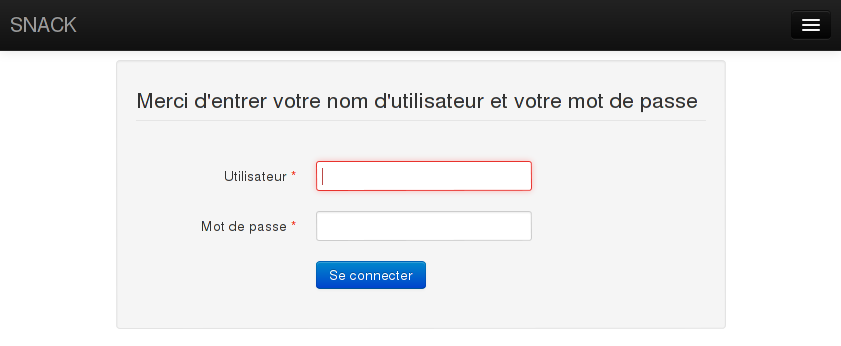
\includegraphics[width=0.9\textwidth]{img/login.png}
	\end{center}
	\caption{Identification sur l'interface.}
	\label{login}
\end{figure}

La première page qui s'affiche correspond à celle des utilisateurs. Comme on peut le voir sur la figure~\ref{general} page~\pageref{general}, l'interface a été conçue en quatre zones~:

\begin{enumerate}
\item Le menu horizontal du haut, qui permet de revenir à l'accueil, de changer l'interface de mode, ou bien de déconnecter l'utilisateur. Puisque l'interface utilise un \emph{responsive design}, ces actions sont regroupées dans une menu déroulant si l'affichage est trop petit (avec un périphérique mobile, par exemplek comme le montre la figure~\ref{responsive} page~\pageref{responsive}).
\item Le menu latéral gauche, qui propose toutes les grandes sections de l'interface, sur lesquelles nous allons revenir plus longuement par la suite.
\item La zone principale qui contient le contenu de la page, selon la section sélectionnée dans le menu de gauche.
\item Le pied de page, qui contient principalement deux boutons à droite, permettant de changer instantanément la langue de toute l'interface. Si l'utilisateur visite l'interface avec un navigateur anglais, l'interface est par défaut en anglais.
\end{enumerate}

\begin{figure}[!h]
	\begin{center}
	    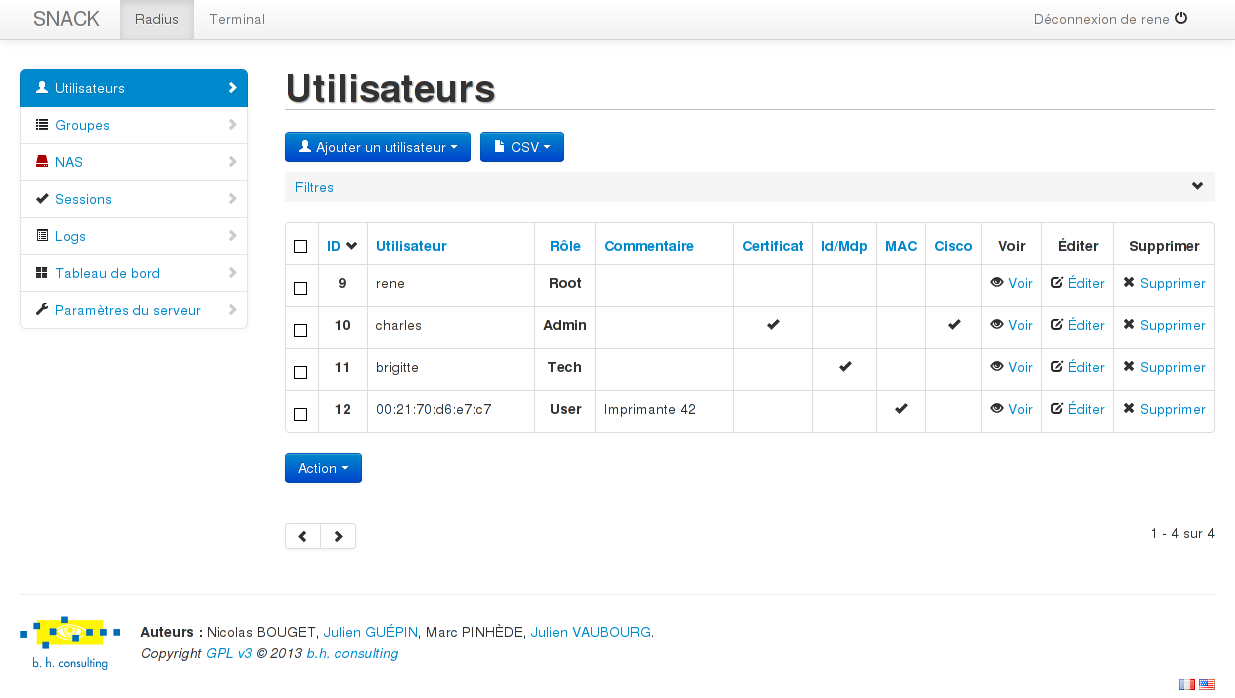
\includegraphics[width=0.9\textwidth]{img/general.png}
	\end{center}
	\caption{Vue générale de l'interface.}
	\label{general}
\end{figure}

\begin{figure}[!h]
	\begin{center}
	    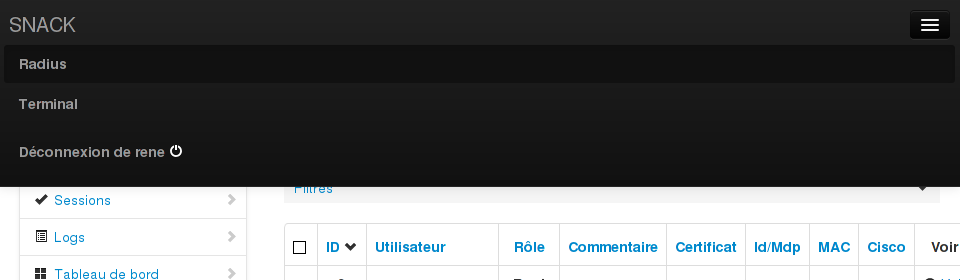
\includegraphics[width=0.9\textwidth]{img/responsive.png}
	\end{center}
	\caption{Responsive design.}
	\label{responsive}
\end{figure}

Comme \textbf{pour toutes les pages qui suivront}, nous retrouvons plusieurs éléments~:

\begin{itemize}
\item La possibilité de faire une recherche dans le tableau, en filtrant très finement les lignes à afficher, grâce au panneau déroulé qui est présenté en figure~\ref{filters} page~\pageref{filters}.
\item Un tableau récapitulatif, pour lequel chaque colonne peut être triée dans un sens comme dans l'autre.
\item La possibilité d'effectuer des actions de masse, en cochant directement les lignes. Cette sélection peut être encore plus rapidement contrôlée en utilisant la touche majuscule du clavier, qui permet d'aller d'une ligne A à une ligne B en cochant toutes les lignes qui sont entre les deux. Un exemple avec l'action \og~Supprimer~\fg (sélectionnable dans le menu du bas) est donné en figure~\ref{massdel} page~\pageref{massdel}.
\item Une pagination, pour un meilleur confort visuel (le nombre d'éléments par page pouvant être réglé dans les options de l'interface).
\end{itemize}

\begin{figure}[!h]
	\begin{center}
	    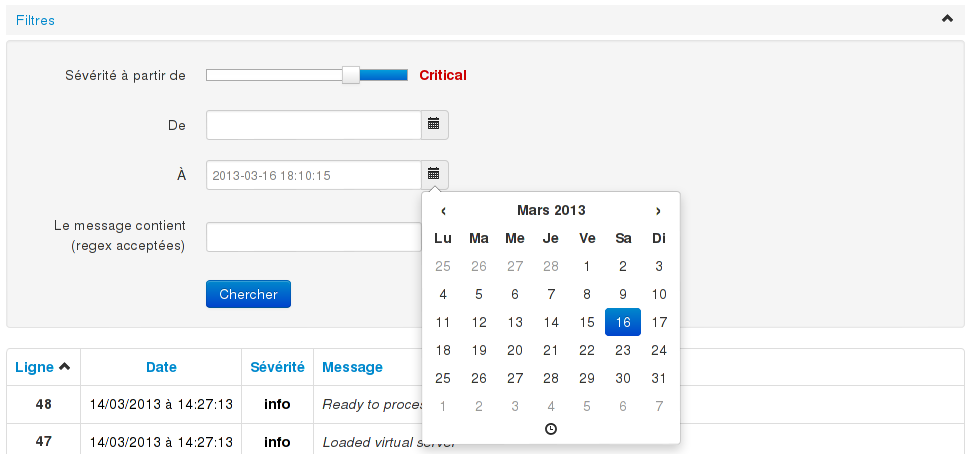
\includegraphics[width=0.9\textwidth]{img/logsfilters.png}
	\end{center}
	\caption{Panneau de recherche.}
	\label{filters}
\end{figure}

\begin{figure}[!h]
	\begin{center}
	    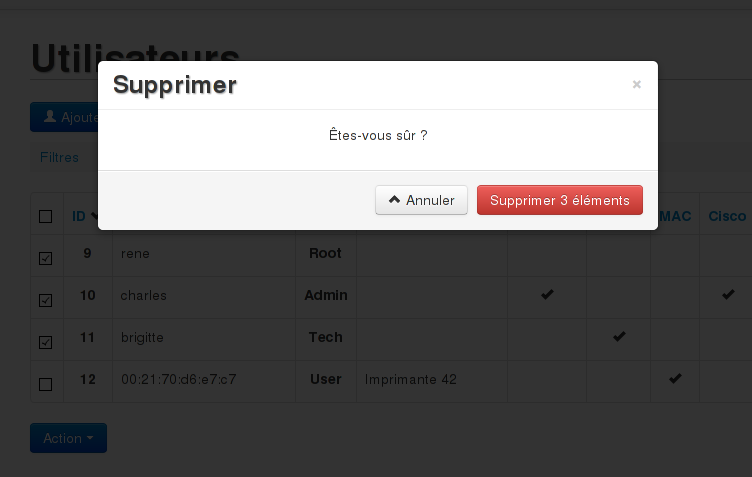
\includegraphics[width=0.6\textwidth]{img/massdel.png}
	\end{center}
	\caption{Suppression multiple.}
	\label{massdel}
\end{figure}

Les prochaines sections détaillent les possibilités offertes par l'interface, en suivant l'ordre des choix du menu latéral.

\subsection{Gestion des utilisateurs}

La page affichée dans la figure~\ref{general} page~\pageref{general} correspond à la section du menu \og~Utilisateurs~\fg.

Le tableau au centre présente tous les utilisateurs créés depuis la mise en route de l'interface, avec leurs caractères les plus pertinents. Plus d'informations par utilisateur peuvent être affichées, en visualisant leur page personnelle.

Le menu principal (figure~\ref{menuusers} page~\pageref{menuusers}) de la page \og~Ajouter un utilisateur~\fg{} propose trois types d'utilisateur~:

\begin{enumerate}
\item \textbf{Actif~:} Un utilisateur actif est un utilisateur qui s'authentifie sur le réseau de façon pro-active, avec un logiciel d'authentification (éventuellement intégré dans le système d'exploitation). C'est le cas de toutes les machines qui sont suffisamment puissantes et qui peuvent être contrôlées par un humain. L'authentification peut se faire par certificat (authentification forte en vert) ou par identifiant et mot de passe (authentification plus faible en orange).
\item \textbf{Passif (MAC)~:} Contrairement à l'utilisateur actif, le passif n'a pas conscience de s'authentifier sur le réseau. C'est donc la seule information qu'il transmet qui est utilisée pour le reconnaître, son adresse MAC. Cette authentification est très faible (il est facile d'usurper une adresse de ce type), mais il correspond parfaitement à des équipements comme les imprimantes qui ne savent pas s'authentifier de façon pro-active. Ce genre d'équipement a aussi l'avantage de n'avoir en général accès qu'à un réseau virtuel très limité (ce qui est configurable via SNACK).
\item \textbf{Snack~:} Ce dernier type d'utilisateur correspond à un utilisateur qui a le droit d'accéder à l'interface de SNACK. Nous verrons qu'il peut évidemment être recoupé avec d'autres fonctions, pour être polyvalent.
\end{enumerate}

\begin{figure}[!h]
	\begin{center}
	    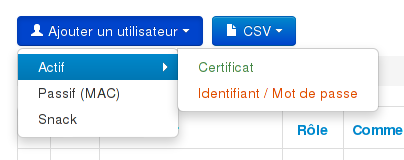
\includegraphics[width=0.5\textwidth]{img/menuusers.png}
	\end{center}
	\caption{Menu d'ajout d'utilisateur.}
	\label{menuusers}
\end{figure}

Cette séparation des utilisateur a été mûrement réfléchie pour permettre à l'interface de s'abstraire des vrais types d'utilisateurs qui existent et qui peuvent se recouper~:

\begin{itemize}
\item Utilisateur s'identifiant sur le réseau en utilisant un identifiant / mot de passe.
\item Utilisateur s'identifiant sur le réseau en utilisant un chiffrement TLS.
\item Utilisateur s'identifiant sur le réseau en utilisant un chiffrement TTLS/PEAP.
\item Utilisateur s'identifiant sur le réseau grâce à son adresse MAC.
\item Utilisateur s'identifiant à la console d'administration des commutateurs avec un identifiant / mot de passe (en Telnet/SSH et/ou console).
\item Utitisateur s'identifiant sur l'interface SNACK avec un identifiant / mot de passe.
\end{itemize}

Ainsi, un utilisateur actif par identifiant / mot de passe, en cochant les options adéquates sur l'interface, pourra s'identifier à la fois sur le réseau et sur les commutateurs avec le même couple d'identifiants s'il le souhaite (et en précisant le type de connexion autorisé).

Il pourra également demander à vérifier le certificat serveur, le passant ainsi automatiquement en chiffrement TTLS pour la partie réseau. Pour encore plus de sécurité, il pourra demander à faire vérifier son adresse MAC, en plus de toutes les autres sécurités.

Les utilisateurs Snack pourront être créé à partir des autres types d'utilisateur (ou non), et réutiliser leurs identifiants préalablement définis pour le réseau et/ou les commutateurs, s'ils le souhaitent. Différents rôles ont été définis pour caractériser les utilisateurs et leur offrir une vision plus ou moins limitée de l'interface~:

\begin{description}
\item[Utilisateur~:] Accès au réseau, pas à l'interface.
\item[Tech~:] Voir les utilisateurs, télécharger les certificats.
\item[Admin~:] Voir, créer, mettre à jour les utilisateurs.
\item[Root~:] Voir, créer, mettre à jour, supprimer tous les objets.
\end{description}

Un type d'utilisateur est absent~: celui qui souhaite être actif et ne s'authentifier que via son adresse MAC. Cette configuration permet d'être plus rapide que le mode passif, qui nécessite l'attente d'un délai d'expiration. Cette option n'a pas été souhaitée par l'entreprise, qui juge que, si les humains ont en effet besoin que ça soit plus rapide que pour les machines, l'authentification par adresse MAC n'est pas souhaitable pour eux étant donné le peu de sécurité que ça apporte.

Par exemple, l'ajout d'un utilisateur qui s'authentifie avec un identifiant et un mot de passe donne lieu à ces différentes options~:

\begin{itemize}
\item Outre le couple utilisateur/mot de passe qui est demandé, l'interface demande si cet utilisateur devra obligatoirement vérifier le certificat serveur pour s'authentifier. Elle demande également une adresse MAC facultative, pour permettre une double-authentification de l'utilisateur. Une date d'expiration peut aussi être positionnée, dans le cas d'un stagiaire, par exemple (résultat dans le tableau, sur la figure~\ref{usersexp} page~\pageref{usersexp}).
\item Un utilisateur peut appartenir à un ou plusieurs groupes, sélectionnables par glissé-déposé.
\item Comme l'illustre la figure~\ref{userscisco} page~\pageref{userscisco}, un utilisateur du réseau peut aussi être un utilisateur qui s'authentifie sur les équipements Cisco. Ainsi, l'interface propose d'activer cette possibilité pour cet utilisateur, en proposant de contrainte le mode de connexion (Telnet/SSH, Console ou les deux).
\item Un numéro de réseau virtuel peut être automatiquement répondu lorsque cet utilisateur se connecte. Ainsi, il sera automatiquement contraint à des accès spécifiques.
\item Et enfin son rôle, pour devenir ou non un administrateur de l'interface SNACK.
\end{itemize}

\begin{figure}[!h]
	\begin{center}
	    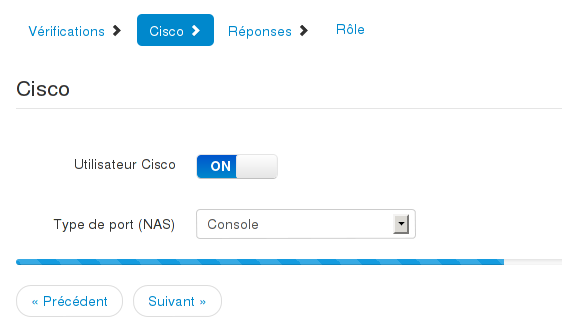
\includegraphics[width=0.6\textwidth]{img/userscisco.png}
	\end{center}
	\caption{Configuration Cisco pour un nouvel utilisateur.}
	\label{userscisco}
\end{figure}

\begin{figure}[!h]
	\begin{center}
	    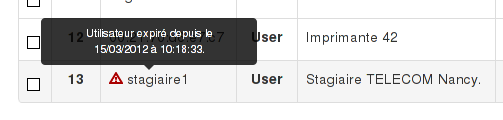
\includegraphics[width=0.6\textwidth]{img/usersexp.png}
	\end{center}
	\caption{Utilisateur expiré.}
	\label{usersexp}
\end{figure}

La copie d'écran ~\ref{userscisco} page~\pageref{userscisco} a permis de mettre en avant l'organisation en étapes avec une barre de progression qu'on retrouve dans toutes les pages de formulaire, pour une meilleure expérience utilisateur.

Un second menu est proposé pour les utilisateurs~: il permet d'importer ou d'exporter des utilisateurs en utilisant un fichier CSV. Cette fonctionnalité permet d'ajouter des utilisateurs en grand nombre, ou d'exporter la base de données. L'exportation peut se faire finement, notamment grâce à la sélection multiple qui permet de choisir les utilisateurs à exporter.

\subsection{Gestion des groupes}

Une autre façon d'automatiser les droits sur le réseau pour un utilisateur est de lui affecter un groupe (figure~\ref{groupes} page~\pageref{groupes}). Ce groupe aura des droits similaires à ceux proposés pour les utilisateurs, et ils ne s'appliqueront que s'ils n'ont pas été positionnés par l'utilisateur. Cette fonctionnalité permet de créer des utilisateurs de façon efficace, en se contentant de les associer à des groupes qui ont été configurés au préalable. Un utilisateur peut être affecté à plusieurs groupes.

\begin{figure}[!h]
	\begin{center}
	    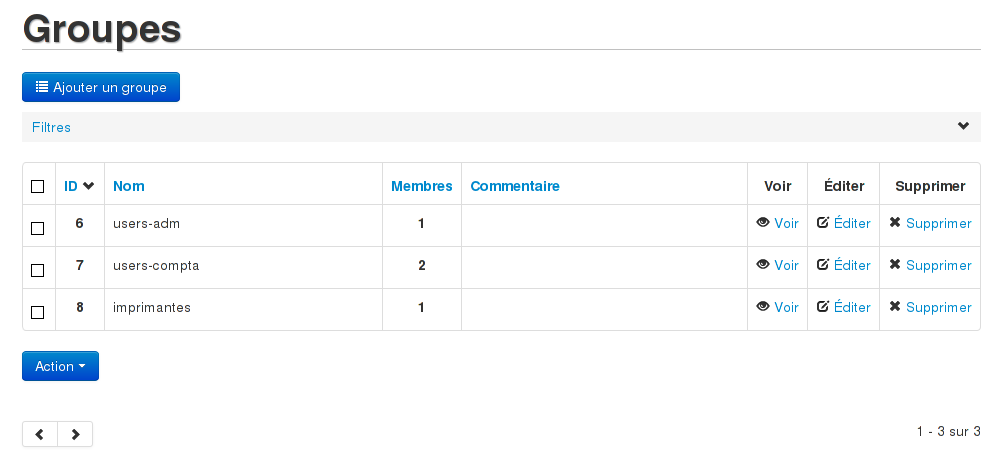
\includegraphics[width=0.9\textwidth]{img/groupes.png}
	\end{center}
	\caption{Gestion des groupes.}
	\label{groupes}
\end{figure}

Un groupe peut également avoir une date d'expiration. La figure~\ref{groupesedit} page~\pageref{groupesedit} illustre l'édition d'un groupe, qui permet entre autres de définir les utilisateurs qui lui appartiennent via des glissés-déposés.

\begin{figure}[!h]
	\begin{center}
	    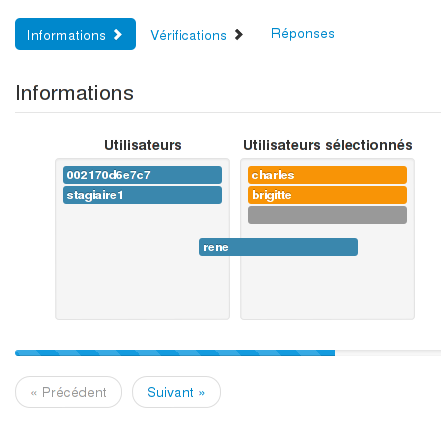
\includegraphics[width=0.5\textwidth]{img/groupesedit.png}
	\end{center}
	\caption{Édition d'un groupe.}
	\label{groupesedit}
\end{figure}

\subsection{Gestion des NAS}

Comme on peut l'apercevoir dans la figure~\ref{nas} page~\pageref{nas}, un commutateur n'est caractérisé que par quatre paramètres~:

\begin{enumerate}
\item Son nom.
\item Son IP.
\item Sa clé secrète.
\item Une description.
\end{enumerate}

\begin{figure}[!h]
	\begin{center}
	    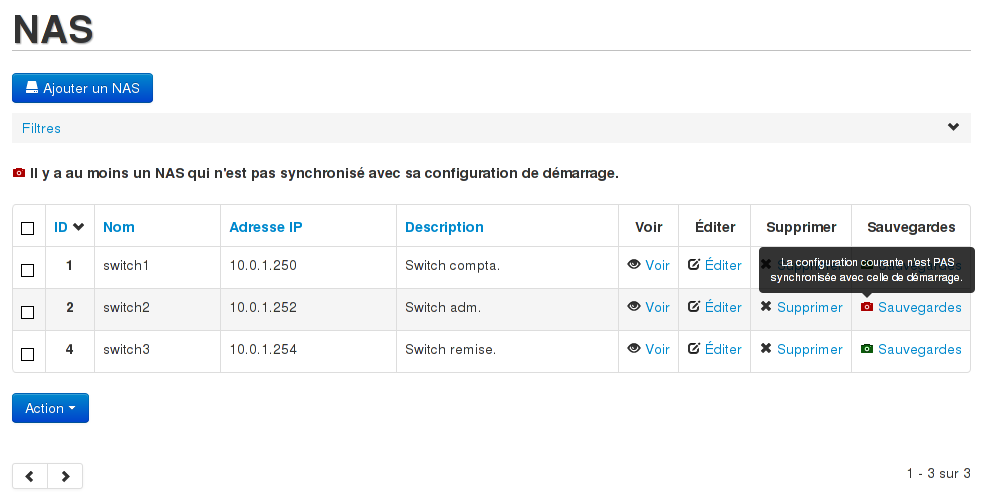
\includegraphics[width=0.9\textwidth]{img/nas.png}
	\end{center}
	\caption{Liste des commutateurs.}
	\label{nas}
\end{figure}

La ligne en dessous du panneau des filtres indique qu'un des commutateurs a eu des changements dans sa mémoire, sans qu'ils ne soient synchronisés avec sa configuration de démarrage. Si ces changements ont bien été sauvegardés automatiquement dans l'interface, le commutateur ne la chargera pas s'il redémarre. Il est donc important de préciser à l'utilisateur qu'il a fait un oubli de grande importance.

Par ailleurs, l'icône de la section NAS change de couleur selon si tous les commutateurs sont synchronisés ou non (figure~\ref{menunas} page~\pageref{menunas}).

La dernière colonne permet d'accéder à la liste des sauvegardes automatisées qui ont eu lieu. La section suivante en explicite le contenu.

\begin{figure}[!h]
	\begin{center}
	    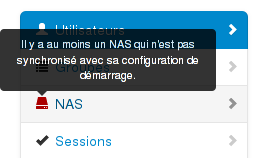
\includegraphics[width=0.3\textwidth]{img/menunas.png}
	\end{center}
	\caption{L'icône est verte ou rouge selon si tous les commutateurs sont synchronisés ou non.}
	\label{menunas}
\end{figure}

\subsection{Gestion des sauvegardes}

Un exemple de liste des sauvegardes automatiques pour un commutateur est donnée en figure~\ref{backups} page~\pageref{backups}.

\begin{figure}[!h]
	\begin{center}
	    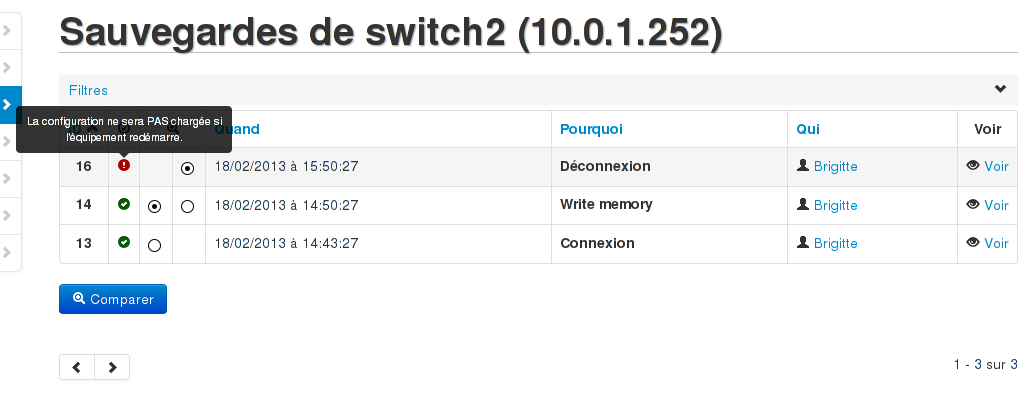
\includegraphics[width=0.9\textwidth]{img/backups.png}
	\end{center}
	\caption{Liste des sauvegardes pour un commutateur.}
	\label{backups}
\end{figure}

Cette liste montre qu'il y a eu trois sauvegardes, avec des modifications de la configuration du commutateur, entre chacune. On peut constater qu'il s'agit d'un cycle classique de connexion, écriture et déconnexion. Mais on constate grâce aux icônes de couleur, que Brigitte a fait des modifications dans la configuration depuis sa dernière écriture, et a quitté sans synchroniser. Elles sont donc sauvegardées sur le serveur, mais le commutateur ne les prendra pas en compte en cas de redémarrage.

Pour mieux comprendre les changements, l'interface permet de comparer chacune des versions, avec un affichage convivial visible dans la figure~\ref{backupsdiff} page~\pageref{backupsdiff}.

\begin{figure}[!h]
	\begin{center}
	    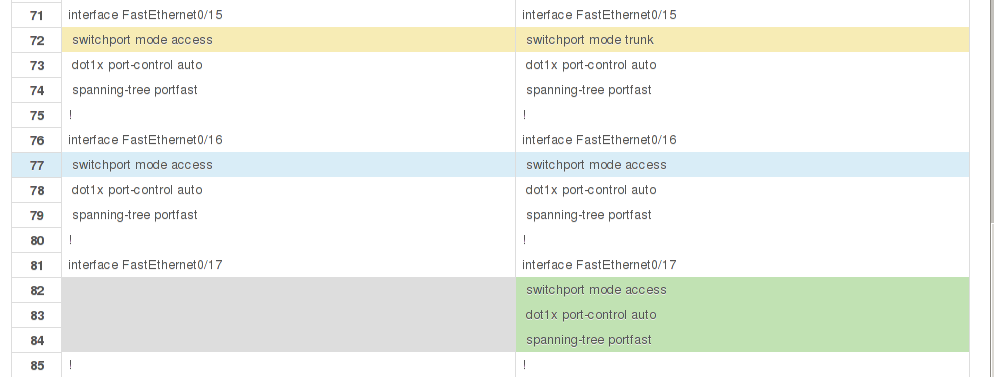
\includegraphics[width=0.8\textwidth]{img/backupsdiff.png}
	\end{center}
	\caption{Comparaison entre deux sauvegardes.}
	\label{backupsdiff}
\end{figure}

En affichant une sauvegarde, comme l'illustre la figure~\ref{backupsview} page~\pageref{backupsview}, trois parties principales se dégagent~:

\begin{enumerate}
\item La comparaison avec la configuration courante du commutateur, si la sauvegarde visualisée n'est pas la plus récente (acec un affichage coloré des différences).
\item La vue \emph{in extenso} de la configuration, à cette version. Dérouler ce panneau permet en plus d'accéder à un bouton pour restaurer la configuration sur le commutateur.
\item Si d'autres sauvegardes automatiques ont eu lieu mais que la configuration n'a pas changée depuis la dernière sauvegarde, elles sont listées dans le tableau de la dernière partie (et invisibles depuis la liste des sauvegardes du commutateur).
\end{enumerate}

\begin{figure}[!h]
	\begin{center}
	    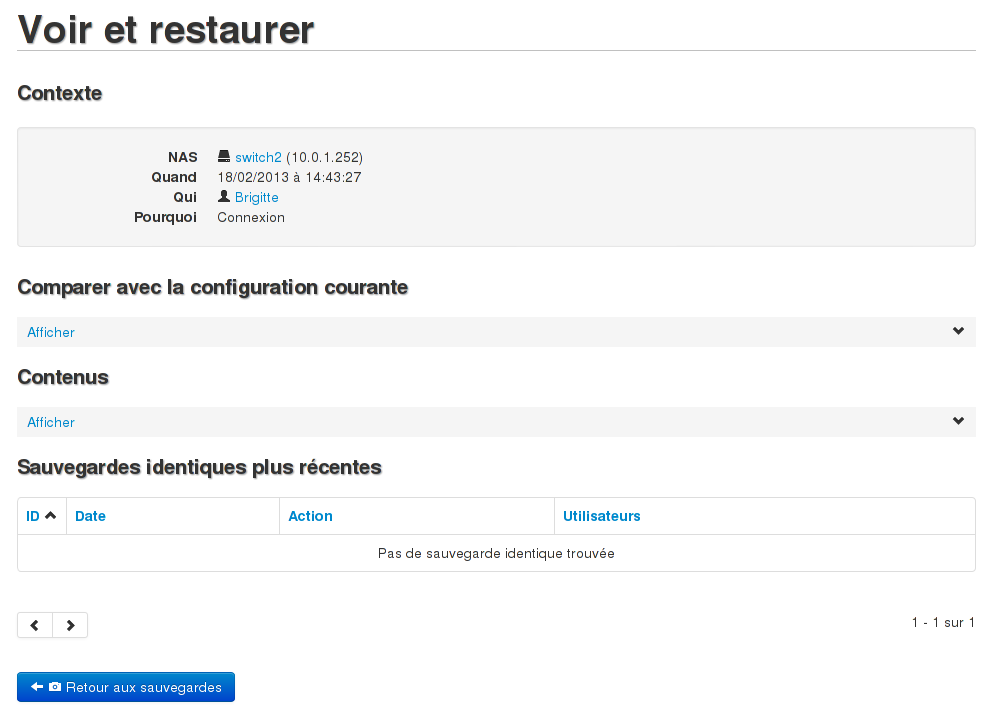
\includegraphics[width=0.9\textwidth]{img/backupsview.png}
	\end{center}
	\caption{Visualisation d'une sauvegarde.}
	\label{backupsview}
\end{figure}

\subsection{Gestion des sessions}

La figure~\ref{sessions} page~\pageref{sessions} présente une liste de sessions enregistrées.

\begin{figure}[!h]
	\begin{center}
	    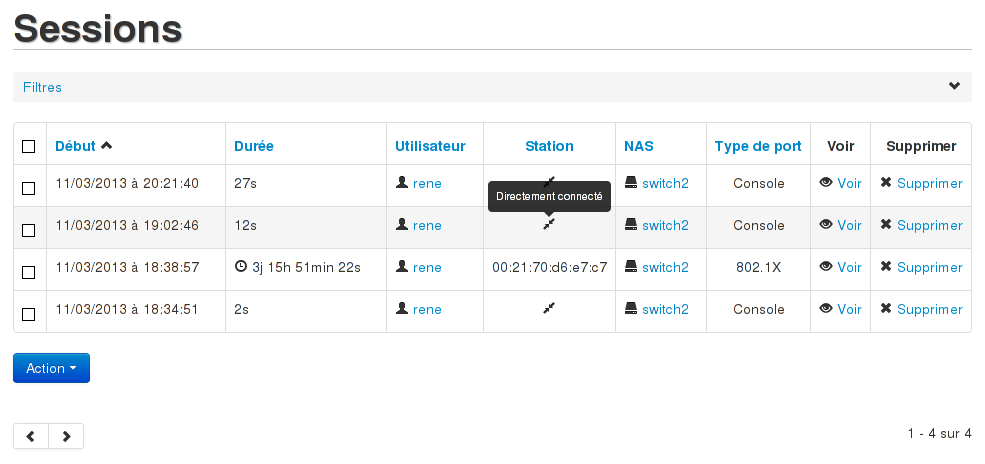
\includegraphics[width=0.9\textwidth]{img/sessions.png}
	\end{center}
	\caption{Visualisation d'une sauvegarde.}
	\label{sessions}
\end{figure}

Que ça soit des authentifications pour de l'administration sur un commutateur, un utilisateur qui se connecte, ou un utilisateur qui se connecte en série au commutateur, tout est enregistré. On peut apercevoir sur la copie d'écran~\ref{sessions} que la troisième session affiche une petite horloge à côté de sa durée. Le temps de connexion est mis à jour dynamiquement en temps réel sur l'interface, pour signifier à l'administrateur que cette session n'est pas encore terminée. Puisque le type de port correspond à du 802.1x, on peut en conclure que René est actuellement connecté via le Switch2, et sur le  poste \texttt{00:21:70:d6:e7:c7} et depuis plus de trois jours.

Les autres connexion de l'exemple se sont faîtes avec un lien série, directement sur le commutateur. La vue d'une session donne beaucoup d'informations supplémentaires.

\subsection{Gestion des journaux systèmes}

La figure~\ref{logs} page~\pageref{logs} révèle la présence de deux onglets pour cette page. Le premier permet d'afficher tous les jounaux du Freeradius, tandis que la seconde permet d'afficher tous ceux de l'interface de SNACK.

\begin{figure}[!h]
	\begin{center}
	    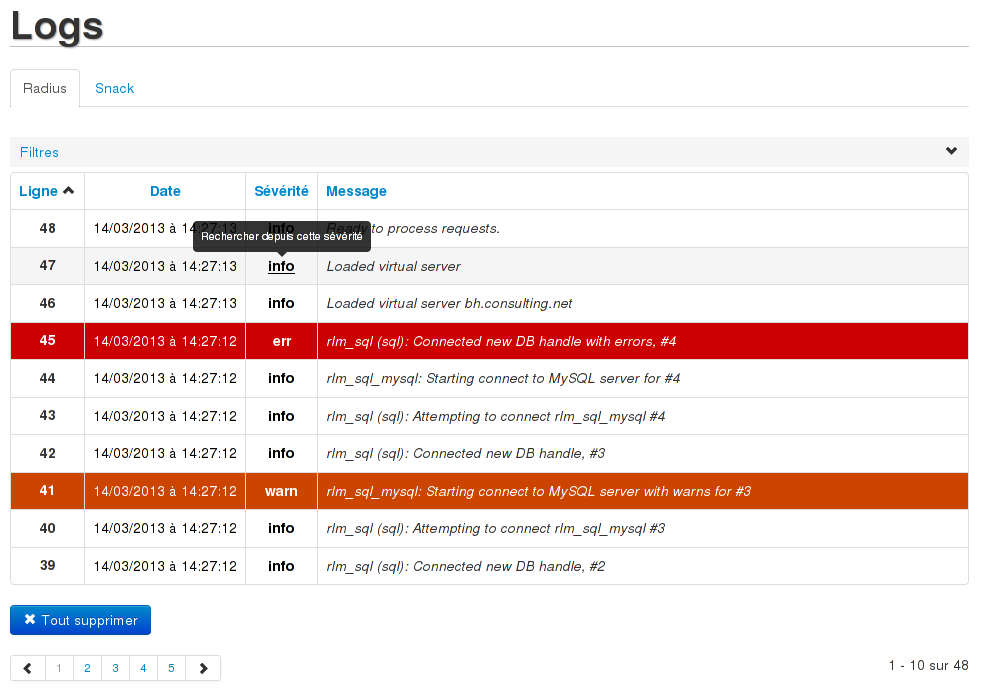
\includegraphics[width=0.9\textwidth]{img/logs.png}
	\end{center}
	\caption{Affichage des journaux systèmes.}
	\label{logs}
\end{figure}

Les lignes sont mises en valeur selon leur gravité, et un puissant outil de filtrage est proposé, via le panneau (comme pour toutes les autres pages) ou directement en cliquant sur les lignes.

\subsection{Tableau de bord}

Le tableau de bord (figure~\ref{dashboard} page~\pageref{dashboard}) est un outil de supervision simplifié du serveur SNACK.

\begin{figure}[!h]
	\begin{center}
	    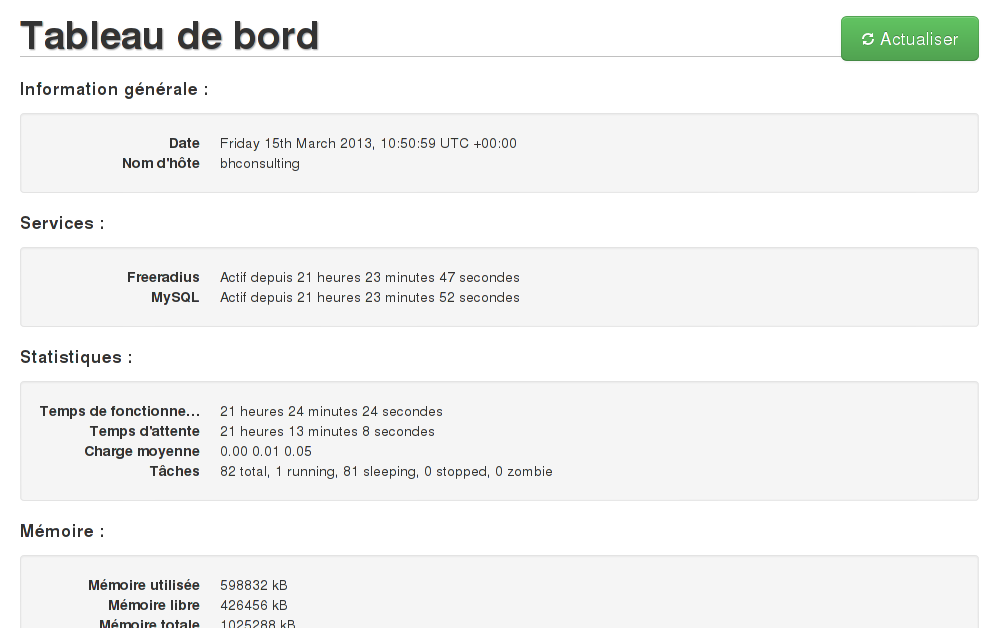
\includegraphics[width=0.9\textwidth]{img/dashboard.png}
	\end{center}
	\caption{Tableau de bord.}
	\label{dashboard}
\end{figure}

Il permet de visualiser~:

\begin{itemize}
\item Des informations générales sur la machine.
\item L'état des deux services principaux que sont Freeradius et MySQL.
\item Des statistiques diverses.
\item L'état des différentes mémoires.
\item L'état des différentes interfaces réseau.
\item Des statistiques détaillées de l'émission et la réception de ces dernières.
\end{itemize}

Il s'agit d'un outil qui pourrait être complété par la suite, notamment en le couplant avec un vrai logiciel de supervision comme Nagios.

\subsection{Paramètres du serveur}

Cette dernière section permet de visualiser et positionner les différents paramètres propres à l'interface de SNACK.

Comme le montre la figure~\ref{parametres} page~\pageref{parametres}, certains paramètres comme la configuration des certificats serviront de valeur par défaut lors de la création de ceux-ci.

\begin{figure}[!h]
	\begin{center}
	    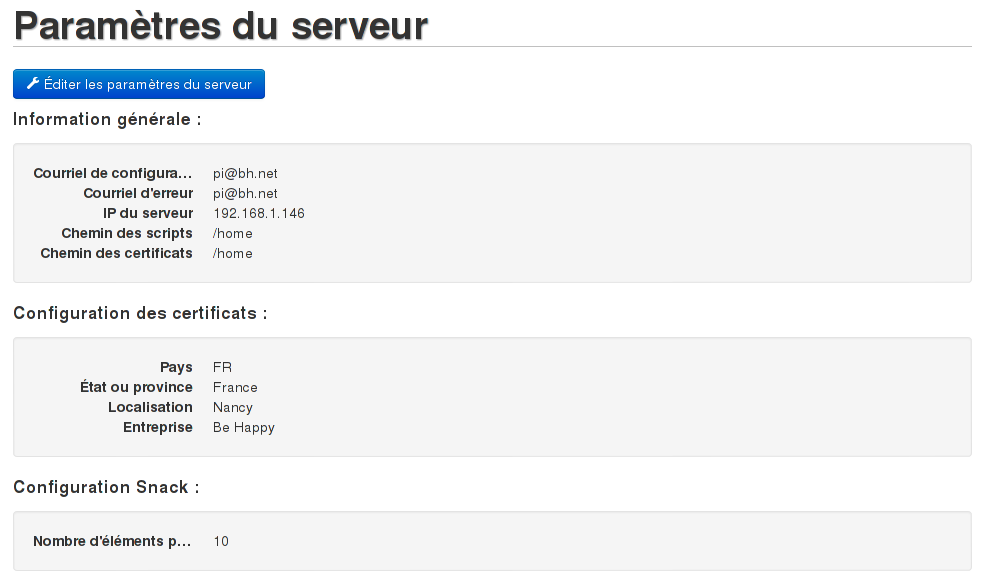
\includegraphics[width=0.9\textwidth]{img/parametres.png}
	\end{center}
	\caption{Paramètres du serveur SNACK.}
	\label{parametres}
\end{figure}

\section{Conclusion}

Que ça soit au niveau gestion de projet ou au niveau technique, ce projet industriel aura été l'occasion pour chacun des membres de l'équipe de découvrir de nombreux outils. La maîtrise de l'interaction entre les protocoles comme la programmation de l'interface ont permis de compléter généreusement la formation d'ingénieur des étudiants, et ont parfois permis de s'aventurer dans des domaines qui n'étaient pas attendus.

Du côté de l'entreprise, le pari semble gagné comme le prouve l'interface finale qui rassemble l'ensemble des fonctionnalités attendues. Le terminal virtuel est une exception, mais son exclusion s'est faite avec l'accord de l'entreprise. Nous conseillons malgré tout à B.H. Consulting de continuer les tests avant de proposer notre solution en production, le temps de développement ayant empiété sur la période d'essai que nous aurions souhaités observer.

B.H. Consulting est maintenant âpte à proposer à ses clients une solution complète, leur permettant de gérer les accès à leurs réseaux et à leurs commutateurs. Grâce à une interface conviviale, cette gestion peut se faire sans connaissances informatiques pointues, et uniquement en ouvrant un navigateur web (dès lors que les commutateurs sont correctement configurés, grâce à la la documentation mise à disposition). Le module de sauvegardes des données tranquilise à la fois les clients et B.H. Consulting, puisque qu'il est désormais possible d'avoir un suivi complet des modifications et de revenir en arrière facilement si nécessaire. Les outils comme la gestion des journaux systèmes, des sessions, la supervision et autres fonctionnalités viennent compléter avantageusement notre solution.

Grâce au paquet d'installation simplifié, un serveur SNACK peut être déployé rapidement et facilement. B.H. Consulting est ainsi capable de proposer des mécanismes complexes en un temps record chez ses clients.

La récente migration du projet en Bootstrap 2.3.1 et en CakePHP 2.3.1\footnote{Il n'y a aucun rapport entre les deux logiciels, c'est donc un hasard si c'est les numéros de leur dernière version sont identiques.} n'a posé aucune difficulté majeure, et prouve que l'interface est écrite proprement et pourra ainsi évoluer facilement dans le futur. Par ailleurs, de nombreuses fonctionnalités pourraient venir compléter notre projet, comme une auto-configuration des commutateurs.

\newpage
~\vspace{5cm}
\begin{center}
	{\Huge \textbf{Annexes}}
\end{center}
\newpage

\appendix

\section{Note de cadrage}
\label{note-cadrage}

\includepdf[pages=-]{note_de_cadrage.pdf}

\section{Cahier des charges}
\label{cahier-charges}
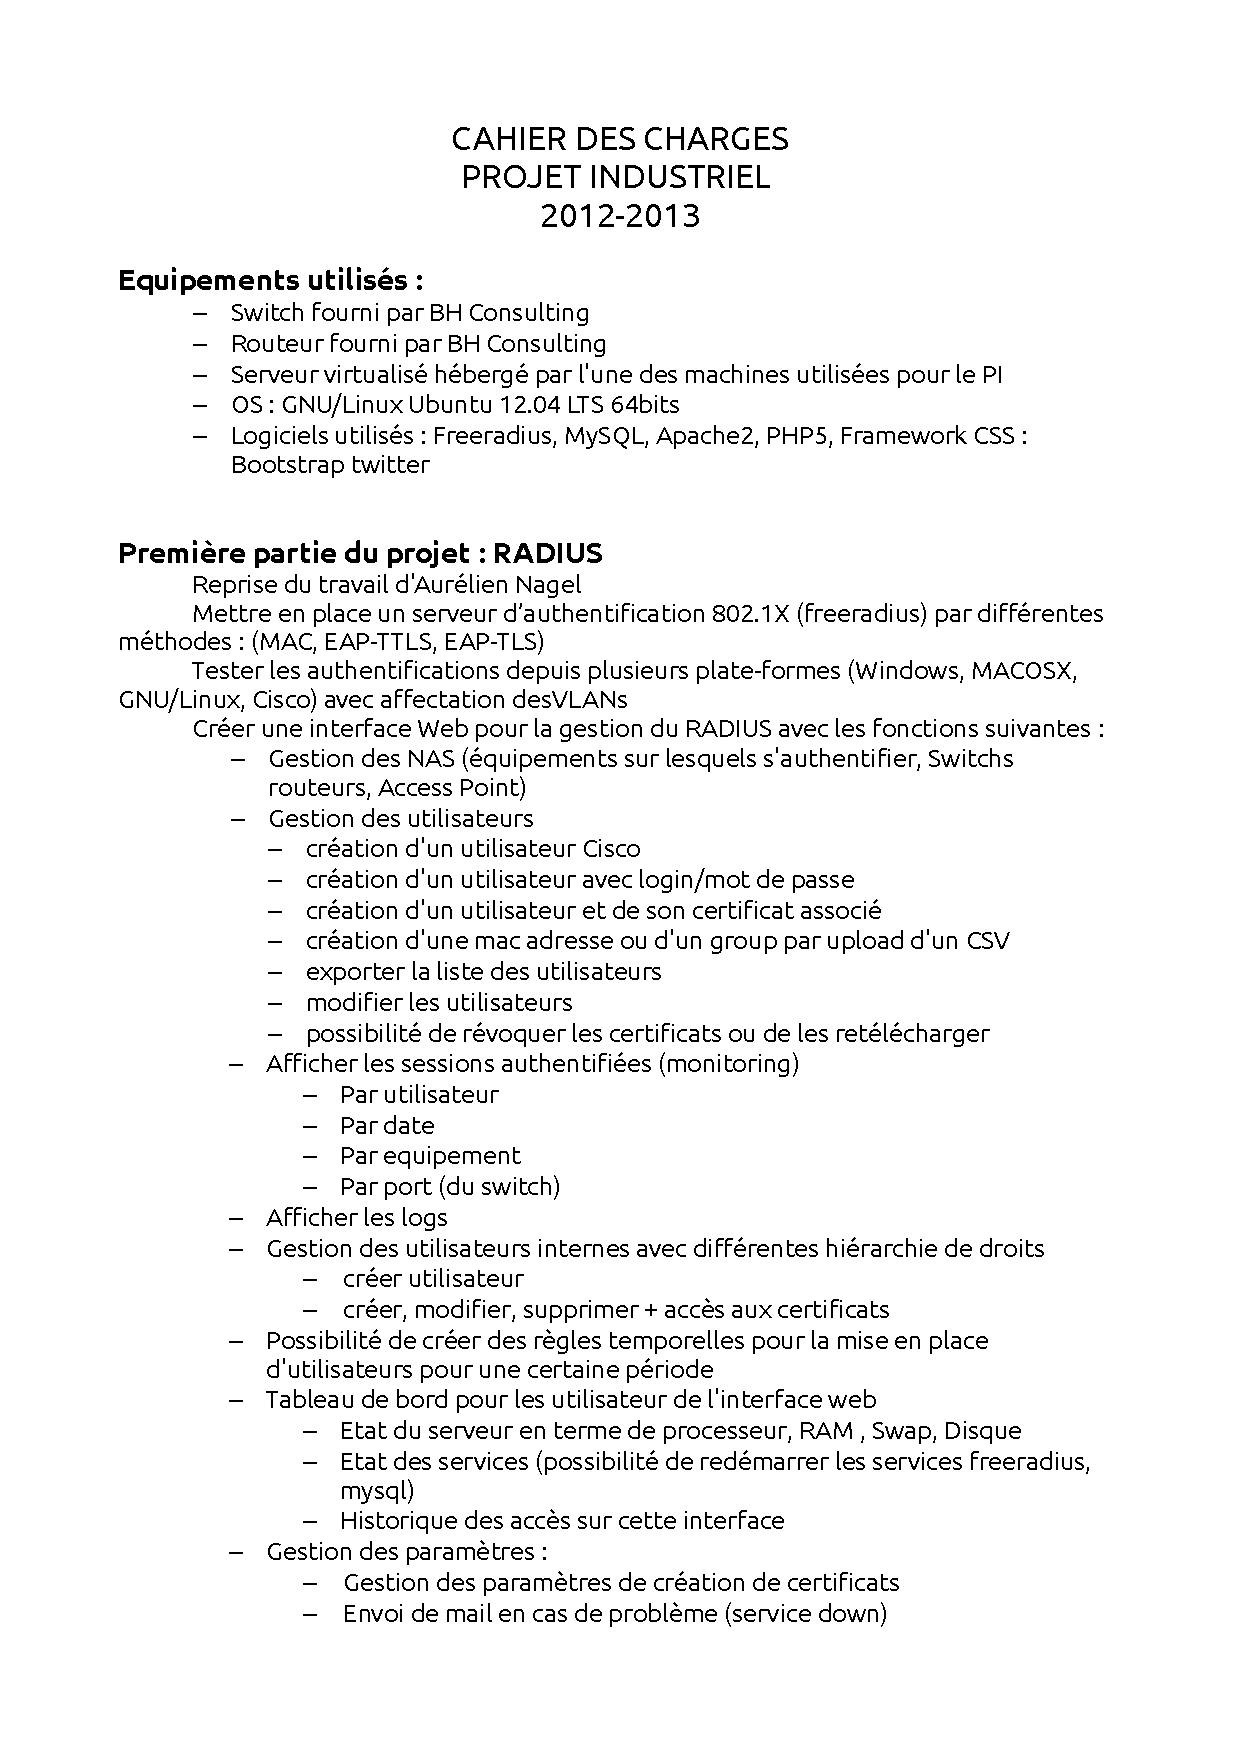
\includepdf[pages=-]{cahier_des_charges.pdf}

\section{Diagramme de Gantt}
\label{gantt}
\begin{center}
	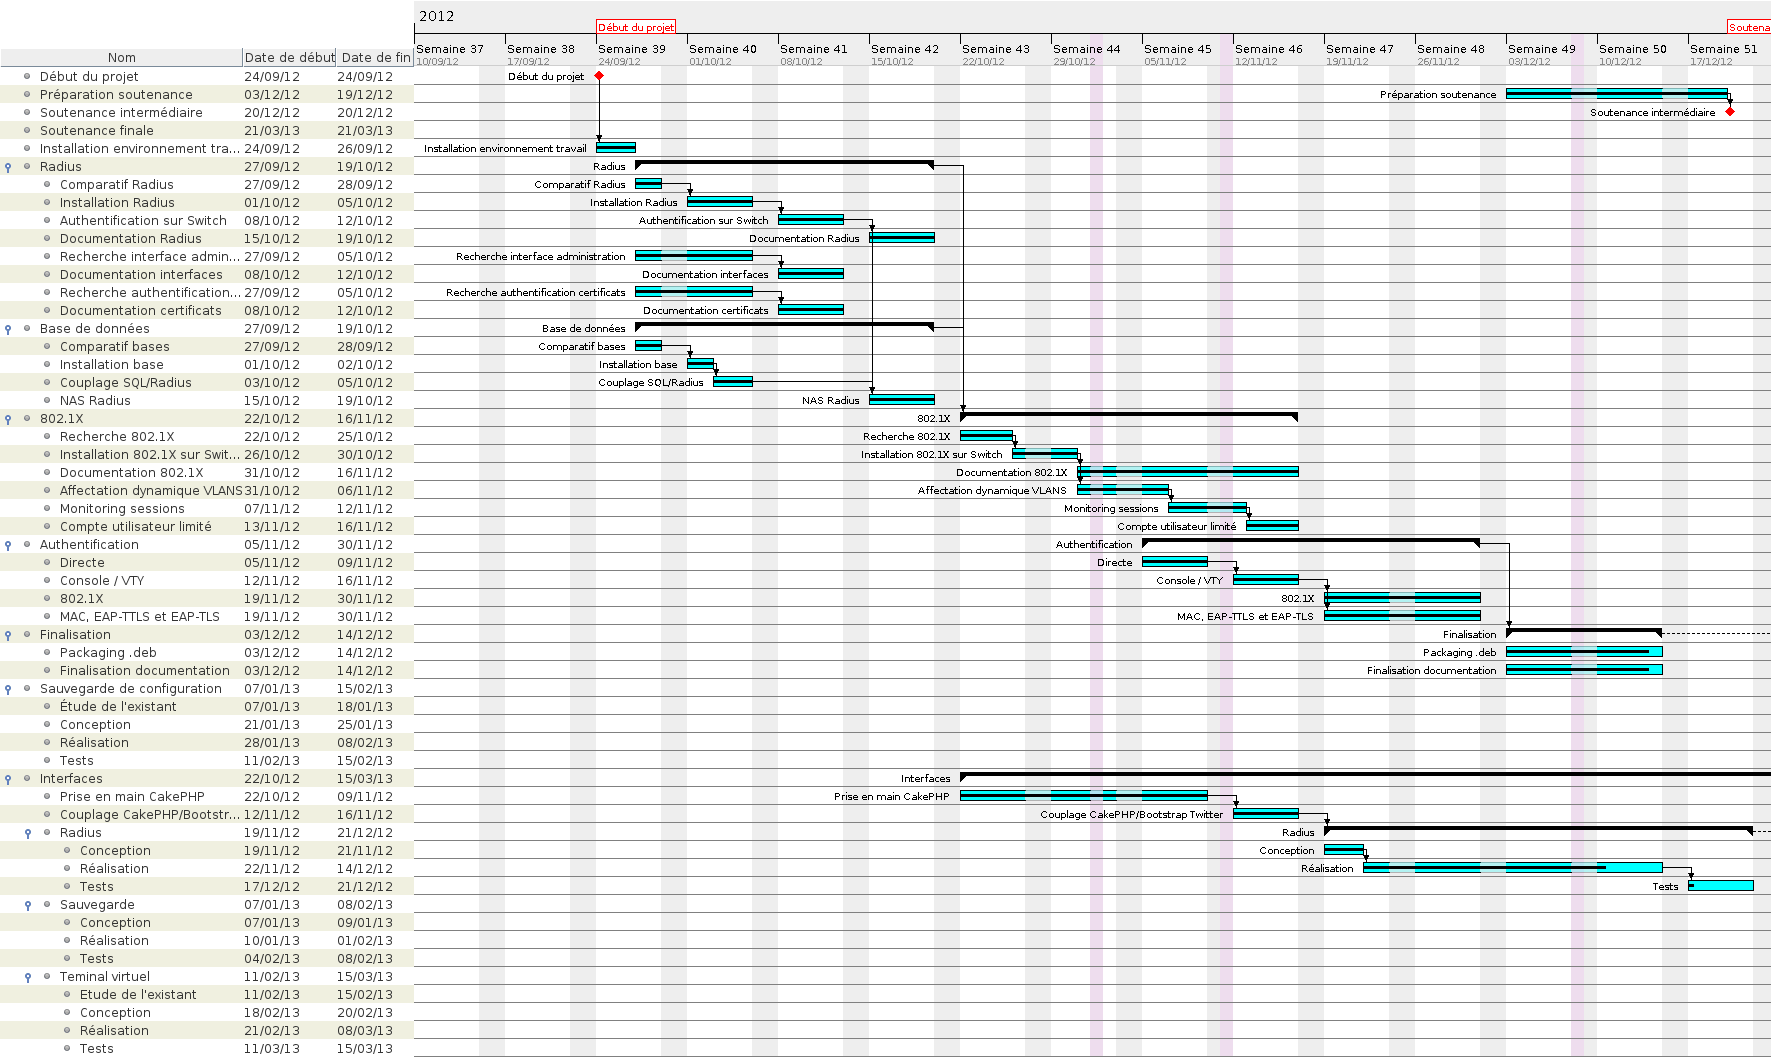
\includegraphics[width=\textwidth]{img/gantt1.png}

	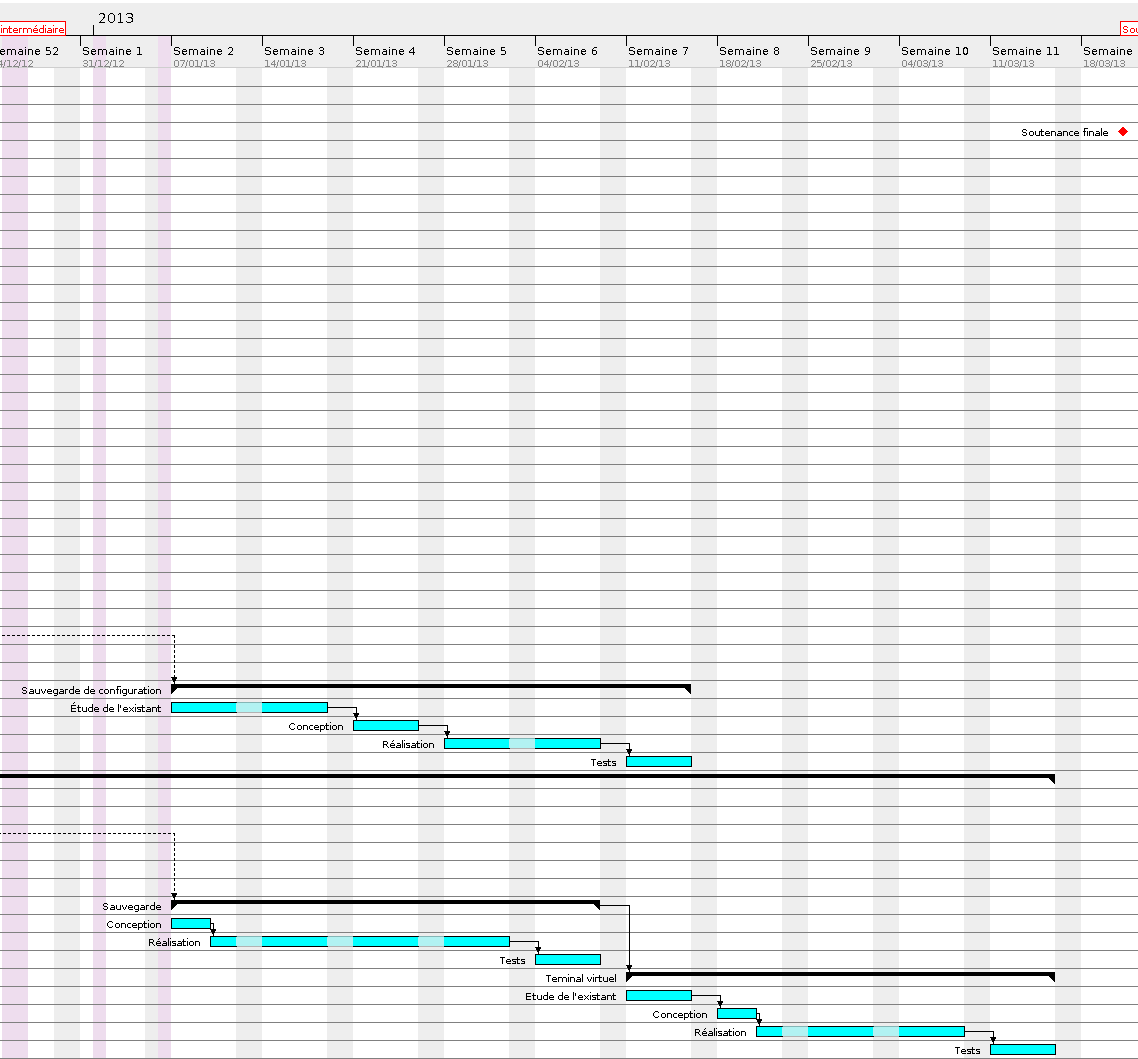
\includegraphics[width=\textwidth]{img/gantt2.png}
\end{center}

\section{Documentation technique}
\label{doc-install}
\includepdf[pages=-]{doc_install.pdf}

\end{document}
